\documentclass[a4paper,marginparwidth=50pt,marginparsep=10pt]{article}
\usepackage{graphicx}
\usepackage{fancyvrb}
\usepackage{listings}
\usepackage{epstopdf}
\usepackage{courier}
\usepackage{hyperref}
\usepackage{mathptmx}
\usepackage{examplep}
\usepackage{cprotect}
\usepackage{calc}
\usepackage{algorithmic}
\usepackage{algorithm}
%margins
% Margin width
\newlength{\marginwidth}
\setlength{\marginwidth}{\marginparwidth}
\addtolength{\marginwidth}{\marginparsep}

\lstset {
basicstyle=\footnotesize\ttfamily,
showstringspaces=false,
numbers=left,
frame=single,
numbersep=5pt,
captionpos=b,
xleftmargin=17pt,
framexleftmargin=17pt,
framexrightmargin=5pt,
framexbottommargin=4pt,
stringstyle=\color{while}\ttfamily,
numberstyle=\tiny
}

\hypersetup{
 colorlinks=true,
 linkcolor=black,
 citecolor=black,
 urlcolor=blue,
}
\DefineVerbatimEnvironment{code}{Verbatim}{fontsize=\normalsize}{\fontfamily{pcr}}
\DefineVerbatimEnvironment{example}{Verbatim}{fontsize=\small}
\hyphenation{free-list Ra-dix-IP-Look-up Pound-Rad-ix-IP-Look-up Bash-Rad-ix-IP-Look-up Read-Rad-ix-IP-Look-up Router-thread}
\begin{document}
\author { 
Madhuri Venkatesh 
\\ UCLA 
\\ \textsl{madhuri@cs.ucla.edu}
\\
\\
\textsl{Supervised By:}
\\Eddie Kohler 
\\ UCLA/Harvard
\\ \textsl{kohler@cs.ucla.edu}
}
\title{Read Copy Update Framework for Userlevel Click}
\maketitle

\pagebreak
\section{Abstract}
High performance routing lookups are critically important for packet forwarding. With multi-core systems becoming more popular and more prevalent, leveraging them is key to improving performance. However, obtaining a correct, scalable and fast thread-safe solution remains challenging.\\

We have described an approach for providing thread-safety using \emph{Read Copy Update}. We have verified that we incur low read side overhead and that our approach performs up to 90\% better than reader-writer locks on read intensive workloads.
\section{Introduction}
The ever-increasing volume of network traffic over the internet demands highly efficient routing lookups. Link rates today exceed 40 Gbps, commodity network cards operate at over 15 Gbps but software routers struggle to comfortably scale beyond 10 Gbps\cite{routebricks}.\\

Commodity machines with SMP multi-core architectures are growing in popularity. A software modular router such as Click\cite{click} running on commodity machines  can benefit greatly by exploiting parallelism on multi-core architectures.\\

Building a scalable and safe multi-core application is not a trivial task. Shared data structures in a multi-threaded application require synchronization for safe and correct access. Synchronization introduces overheads which attenuate the benefits of parallelism. Locks ultimately have the effect of  serialization such that only one thread accesses shared data at a time. A solution using locks also invariably involves the use of variables to synchronize access. These variables need to be accessed simultaneously by other processes or threads causing \emph{cache line bouncing}. This refers to the overhead of communicating the shared value across multiple caches which is very expensive. The larger the number of threads, the greater is the frequency of access of synchronization variables increasing the overall cost of synchronization. The lock based approach becomes less scalable and hence less attractive.\\

We wish to design a highly efficient multi-core solution for IP lookups in a software router. This workload is typically read intensive - comprising of 90\% readers and less than 10\% updaters. \emph{Read Copy Update} (RCU)\cite{readcopyupdate} scales efficiently on read intensive workloads. This is because RCU has very low read side overhead allowing concurrent readers to execute in the presence of a writer without any synchronization. Concurrent writers generally require some form of synchronization. ``RCU permits both readers and writers to make forward concurrent progress''\cite{urcu}. For these reasons, we implemented a Read Copy Update framework for the Click modular router. We compare the performance of our approach against a traditional reader-writer lock and show that RCU does up to 90\% better.\\

The rest of the document is organized as follows. Section \ref{sec:background} gives the reader a background on the userlevel Click elements we are concerned with. Section \ref{sec:problem} describes why implementing a multicore solution was challenging. Section \ref{sec:solution} describes our solutions to the problem along with the implementation details. Sections \ref{sec:perfhypothesis} and \ref{sec:perfeval} describe the performance hypotheses and analysis.
\section{Related Work}
With over 2000 reported uses of the RCU API \cite{rcuusage} in the Linux kernel in recent years, RCU is widely used in system software. It does not seem to be as popular in userlevel applications. Desnoyers et al. \cite{urcu} attribute this to multiple factors such as the constrained design imposed by previous userlevel RCU algorithms, heavy read-side overhead etc. They propose and discuss several approaches to implementing RCU in applications. One such approach is the quiescent state based reclaimation (QSBR)  approach. It has near zero read side overhead but has constraints on application design: it requires that each thread call \verb+rcu_quiescent_state()+ periodically when the thread lies in a quiescent state. Another approach is what is referred to as \emph{General Purpose RCU}. In contrast with QSBR, this approach does not impose any constraints on application design; it can even be used in implementing library functions and API. It has the highest read-side overhead as compared to the other RCU approaches. The overhead is due to memory barriers which are inserted before and after the read side critical sections. The third approach is the \emph{Signal-Based RCU approach}. It avoids the high read-side overhead in the general-purpose approach by sending POSIX signal from the update side critical sections.

Click has natural quiescent states which allow us to implement QSBR. Each thread periodically calls a function which checks for a grace period in order to begin reclaiming stale data. Section \ref{rcuschedloop} describes this mechanism in detail.\\

Hart et al.\cite{hart} compare several different memory reclamation schemes for RCU. Amongst these QSBR is again the scheme with the best performance, but is constrained by the requirement that the application has some natural quiescent states. The authors mention that the QSBR approach can be implemented through a fuzzy barrier. `` A barrier protects access to some code which no thread should execute before all other threads finish some prior stage of computation.''. We describe how we implement the fuzzy barrier in Section\ref{sec:rcu}. The epoch based reclamation (EBR) scheme is application independent, but has higher overhead than QSBR. EBR has some reader side overhead where QSBR has none. EBR uses epochs to implement a fuzzy barrier. Each thread updates local epoch numbers which are checked against a global epoch number to detect quiescent states. Although our approach is modeled on QSBR, it is similar to EBR for several reasons. Firstly, we use epochs to implement a fuzzy barrier. Secondly updaters and \emph{readers} update a local epoch number as opposed to a pure QSBR approach where readers have zero overhead.\\

Dobrescu et al. \cite{routebricks} in \emph{Routebricks} propose an architecture which enables higher packet processing speeds by distributing router functionality across multiple servers and multiple cores within a server. Their approach involves load balancing through Valiant Load Balancing (VLB). Their method of achieving faster packet processing is at a coarser level of granularity when compared to our approach.\\

Multiple efforts have been made at exploiting parallelism in the packet-flow mechanism in a software router. Wu and Wolf \cite{runtimepacketprocessing} have designed a run-time system which distributes the allocation of processing tasks to processor cores. It also balances the workload and maps the it across multiple cores. This parallelism is done at a task-level granularity.\\ 
%It does not look at synchronization of objects being used by the task. In our work we attempt to allow the task itself to be thread-safe so that it can be run on multiple cores.\\

Dobrescu et al. \cite{dobrescu} have proposed a technique in which the packet-processing flow and server characteristics are taken as input to formulate an optimization problem. A compiler would then solve this problem and output machine code which will optimize for throughput.
\section{Background}
\label{sec:background}
This section presents a brief overview of the \emph{RadixIPLookup} element. Our approach involved implementation and analysis using the RadixIPLookup element. We then extended our solution to other elements in Click. 
\subsection{An overview of RadixIPLookup}
The \emph{RadixIPLookup} element \cite{radixiplookup} is a class which is used to perform IP lookups. It uses a radix trie to perform the lookups and a vector to store the routes. This structure is explained in further detail. 
\subsubsection{The Radix Tree}
The radix tree is structured as a trie. The trie has  $2^8$ nodes at the first level, and $2^4$ nodes in the subsequent 6 levels. A lookup therefore has to traverse a maximum of 7 levels. This structure covers all $2^{32}$ IP addresses when the last level is fully occupied. Figure \ref{radixtree} shows the tree pictorially.\\
\begin{figure}[tph]
\begin{center}
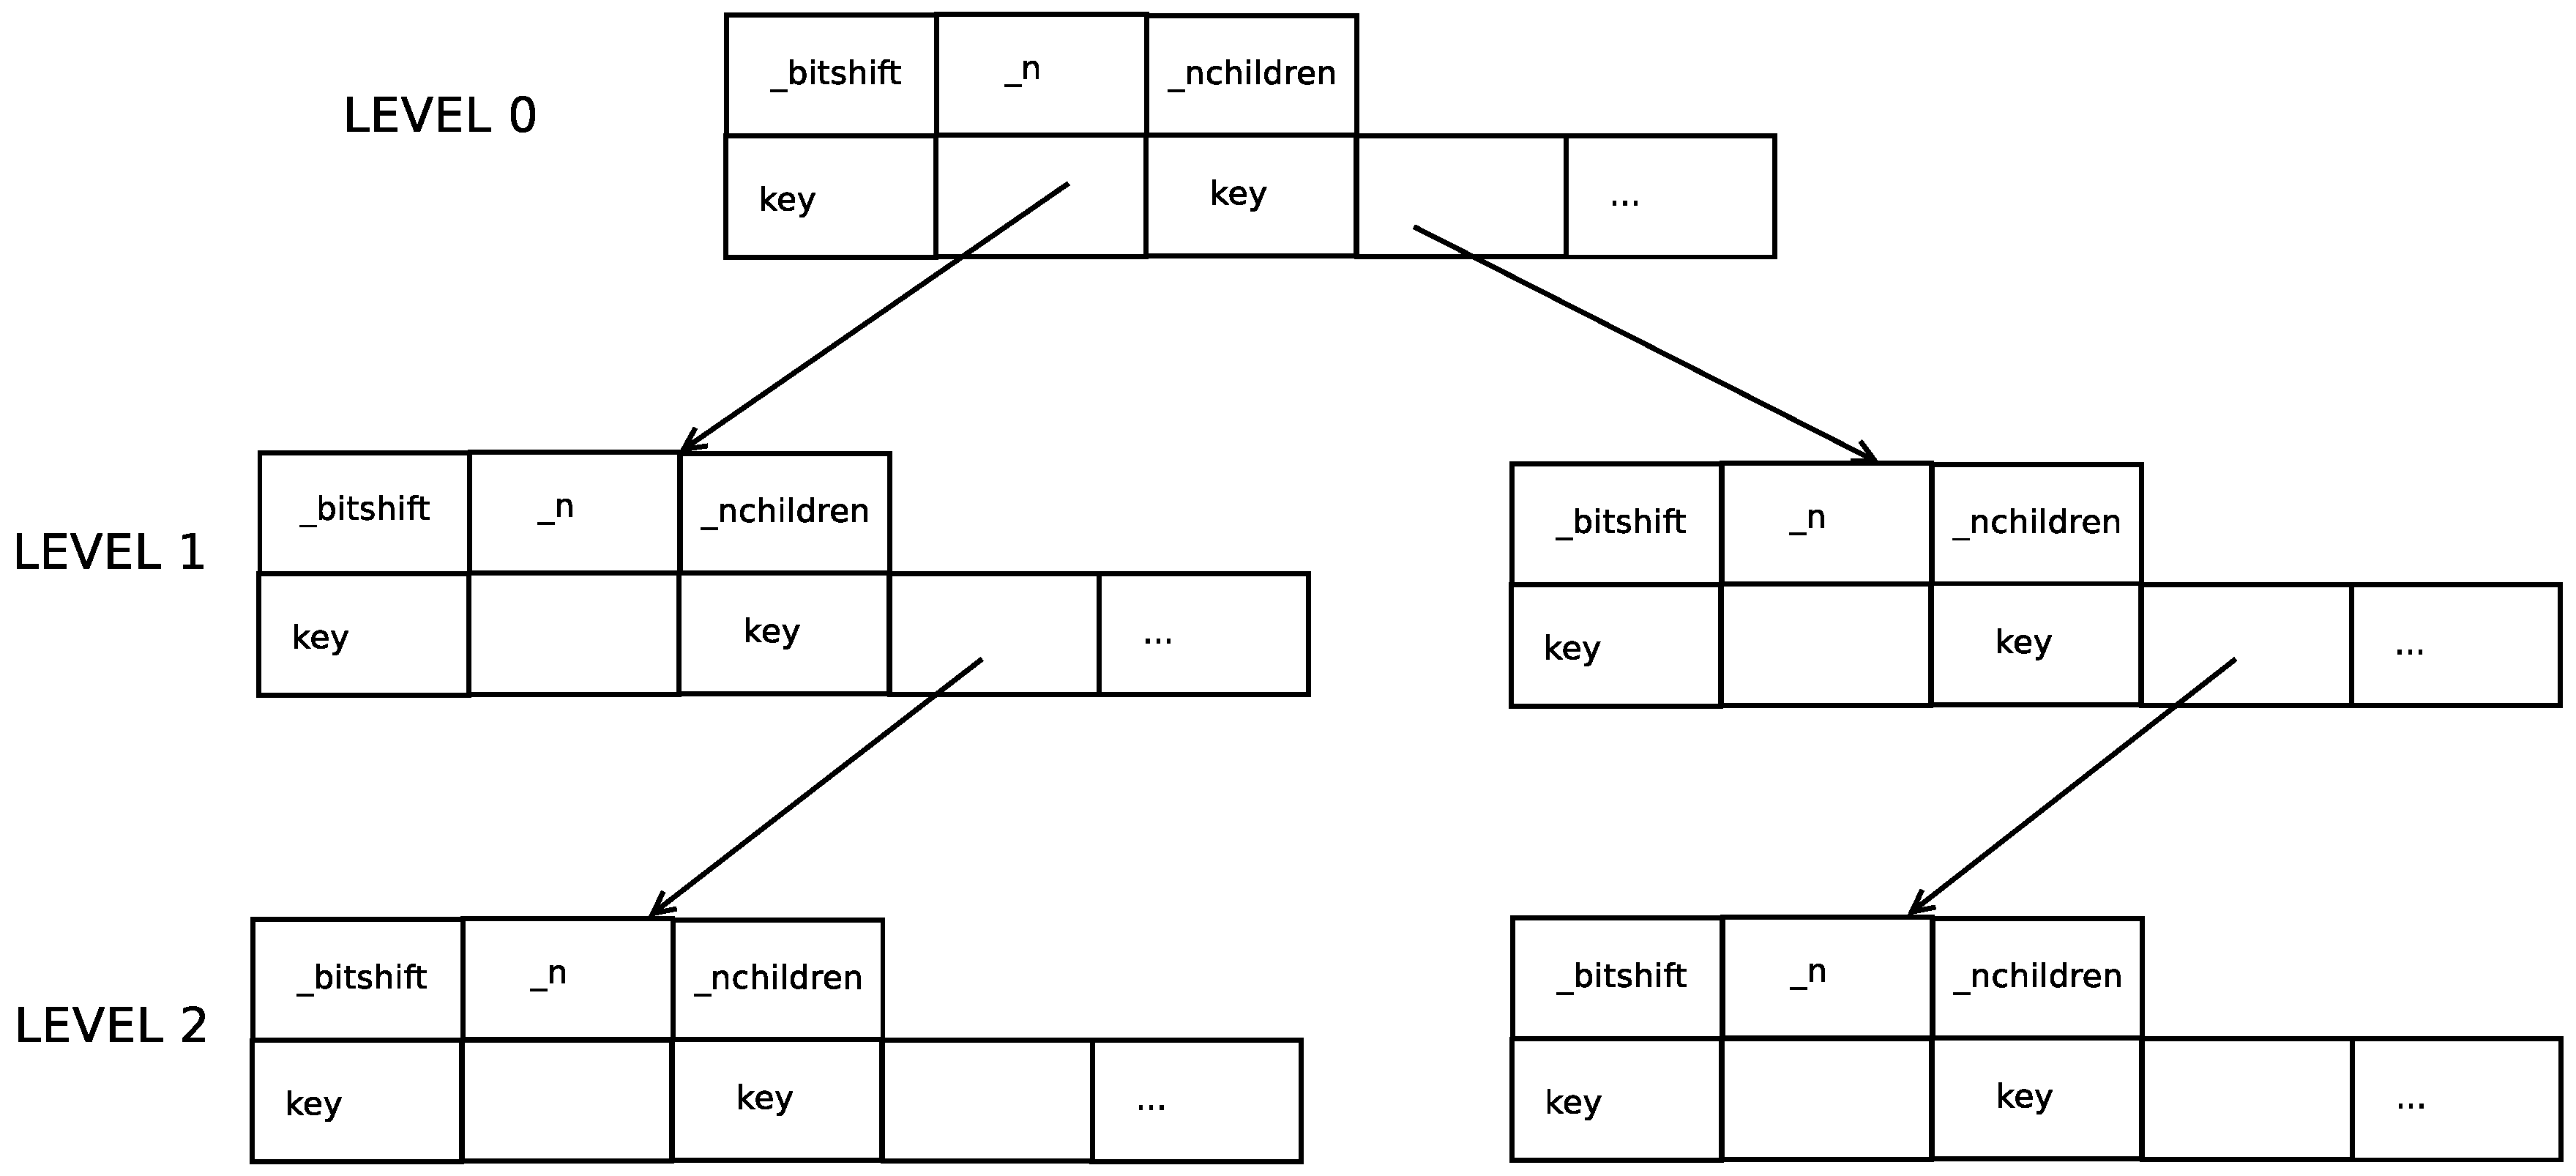
\includegraphics[scale = 0.23]{../images/diagrams/radixtree2.eps}
\caption{The Radix Tree}
\label{radixtree}
\end{center}
\end{figure}
\\Each level consists of radix nodes. The structure of the radix node is shown in Listing \ref{radixnode}. \verb+_n+ represents the number of radix nodes at that level. \verb+_bitshift+ represents the number of bits to be shifted at that level for prefix matching. For the radix node at level 0 \verb+_n+ is 256 and \verb+_bitshift+ is 24 (which is $32 - 8$). This means that the first 8 bits of the address are matched. For the radix nodes at level $1$, \verb+_n+ is 16 and \verb+_bitshift+ is 20 (which is $32 -8 -4$). This means that at level 1, the first 12 bits of the address have been matched.
\begin{lstlisting}[float=tph, caption = The Radix Class, label=radixnode]
class Radix {
  private:

    int _bitshift;
    int _n;
    int _nchildren;
    struct Child {
        int key;
        Radix *child;
    } _children[0];
...
...
}
\end{lstlisting}
The functions \verb+add_route()+ and \verb+delete_route()+ are used to add and delete routes into the routing table.
\paragraph{Lookups}
Routing Table Lookups for the Internet Protocol use a longest prefix match algorithm matching a candidate route with the highest subnet mask. The node at the top most level stores keys which need to match up to an 8 bit long prefix. The nodes in the next level store keys for routes which need to match up to a $12$ bit long prefix and so on. The last level stores keys which can match up to a $32$ bit long prefix. Listing \ref{lookup} shows the code for the lookup. Given an IP Address \emph{addr} which we need to lookup, we calculate the child pointer of the radix node which we need to follow using the \emph{bitshift} at that level. If the key for that child exists we repeat the process trying to obtain the longest prefix match. If it does not exist, we have found the longest prefix match for that node, so we return the key value. This key indexes into a vector which will return the gateway and port for the address.
\begin{lstlisting}[caption = The lookup function, label=lookup]
  static inline int lookup(const Radix *r, int cur, 
                           uint32_t addr) {
    while (r) {
      int i1 = (addr >> r->_bitshift) & (r->_n - 1);
      const Child &c = r->_children[i1];
      if (c.key)
      cur = c.key;
      r = c.child;
    }
    return cur;
  }
\end{lstlisting}
\subsubsection{The Vector class}
The Click library files provide an implementation of a generic Vector. A brief explanation of the use of the vector class in RadixIPLookup is described here. The RadixIPLookup element uses a vector of type IPRoute. IPRoute is a quintuple consisting of \emph{address}, \emph{mask}, \emph{gateway}, \emph{port} and \emph{extra}. Address is the IP adress of the route. Mask is the subnet mask for that route. Gateway is the destination to which a packet matching an address/mask will be routed to through the port. Extra is used to recycle previously used but currently unused space within the vector. It is used to maintain a list of unused entries in the vector. We call this list the \emph{freelist}. If the index in the vector is currently in use extra is set to $-1$, otherwise it stores the index of the next entry in the freelist. If an entry in the vector is deleted, the index of that entry is added to a freelist. Table \ref{tbl:vector} represents a sample vector.

\begin{table}[float=tph]
\begin{center}
\begin{tabular}{|l|l|l|l|l|l|}
\hline index & addr & mask & port & gw & extra\\ 
\hline 0 & 0.0.0.1 & 255.255.255.0 & 1& 22.34.198.3 & 1\\ 
\hline 1 & 1.1.0.1 & 255.255.255.0 & 1& 1.34.198.3 & 5\\
\hline 2 & 2.2.2.1 & 255.255.255.0 & 1& 2.34.198.3 & -1\\
\hline 3 & 1.0.0.1 & 255.255.255.0 & 1& 9.34.198.3 & -1\\
\hline 4 & 4.0.0.1 & 255.255.255.0 & 1& 8.34.198.3 & -1\\
\hline 5 & 4.0.0.1 & 255.255.255.0 & 1& 133.34.198.3 & 3\\
\hline
\end{tabular}
\end{center}
\caption{Sample vector with routes}
\label{tbl:vector}
\end{table}

\begin{figure}[tph]
\begin{center}
\begin{tabular}{|p{2.5in} c|}
\hline
\textbf{State 1}: Initial state of the vector. The freelist reads \{\verb$_vfree =0$, $0\rightarrow1\rightarrow5\rightarrow3$\}. & \raisebox{2ex - \height}{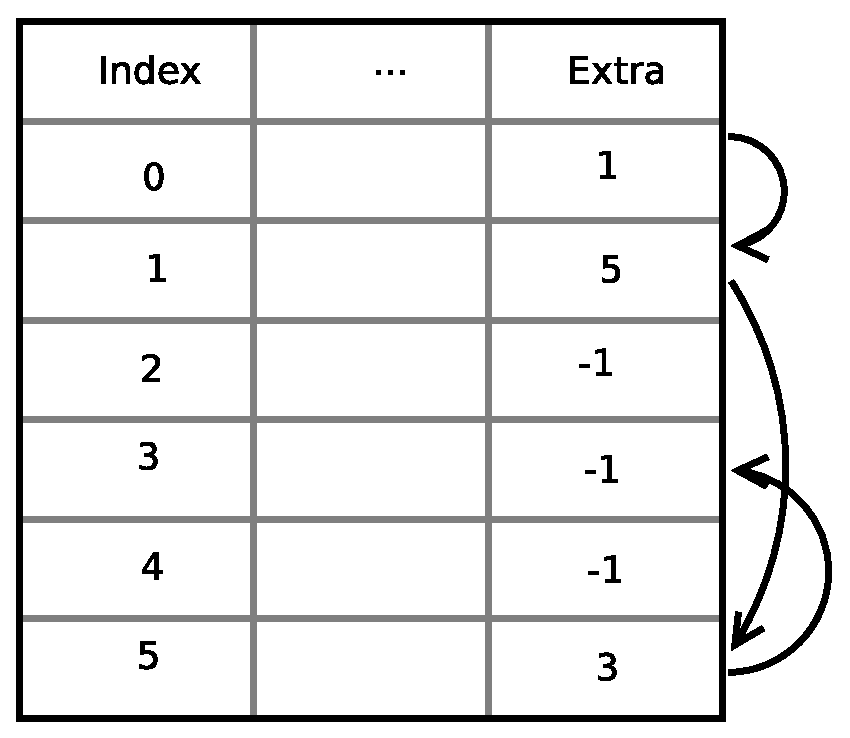
\includegraphics[width=2in,scale=0.4]{../images/diagrams/freelist1.eps}} \\
\hline
\textbf{State 2}: A route is inserted. The index 0 is reused. The freelist reads \{\verb$_vfree =1$, $1\rightarrow5\rightarrow3$\}.& \raisebox{2ex - \height}{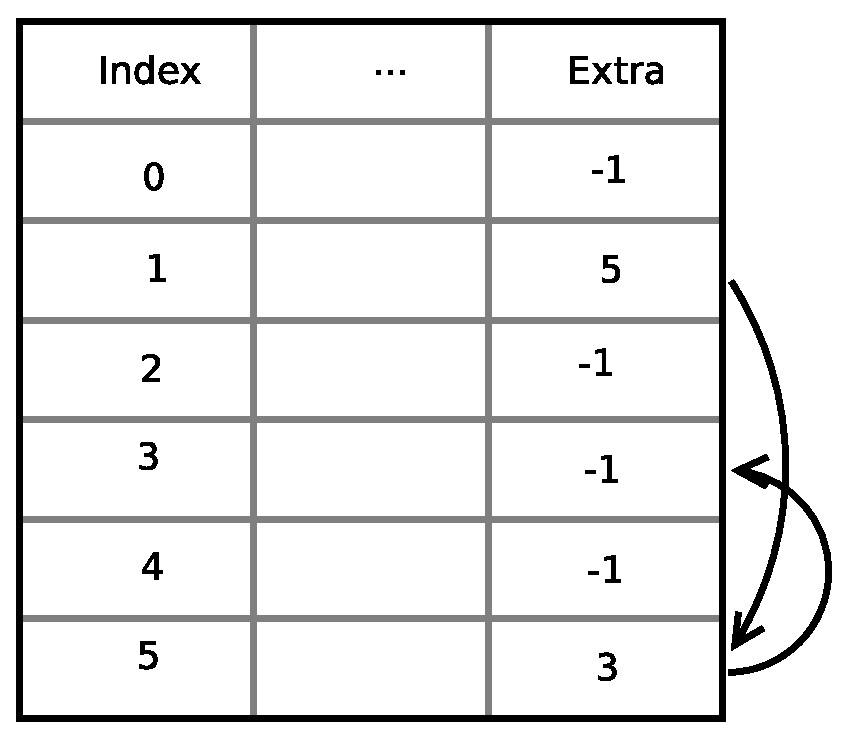
\includegraphics[width=2in,scale=0.4]{../images/diagrams/freelist2.eps}} \\
\hline		
\textbf{State 3}: Another route is inserted. The freelist now reads \{\verb$_vfree =5$, $5\rightarrow3$\}.& \raisebox{2ex - \height}{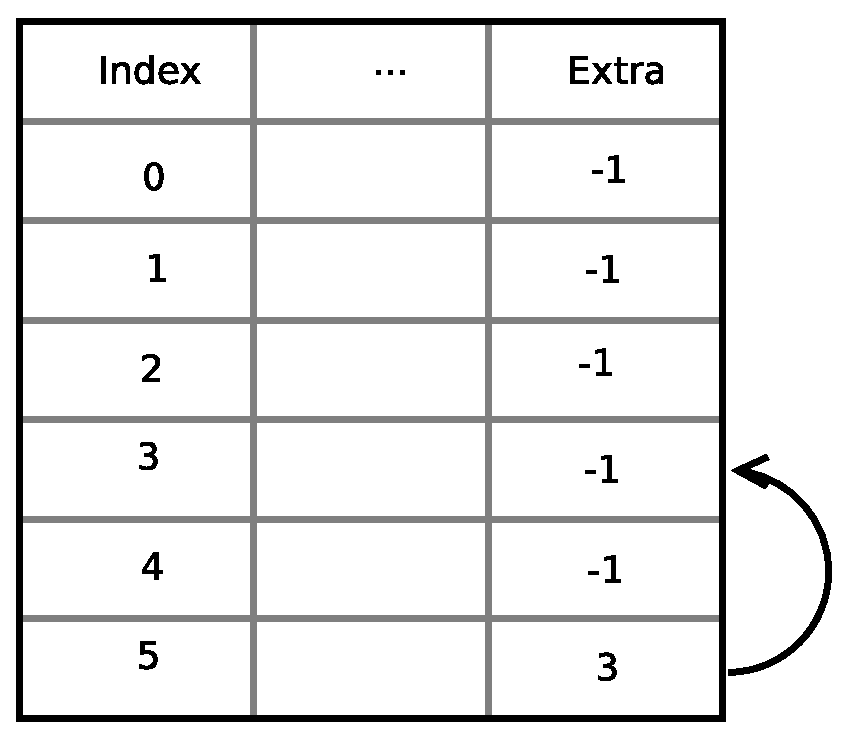
\includegraphics[width=2in,scale=0.4]{../images/diagrams/freelist3.eps}} \\
\hline		
\textbf{State 4}: Route located at index 2 is removed from the vector. Index 2 is added to the freelist. The freelist now reads \{\verb$_vfree =2$, $2\rightarrow5\rightarrow3$\}.& \raisebox{2ex - \height}{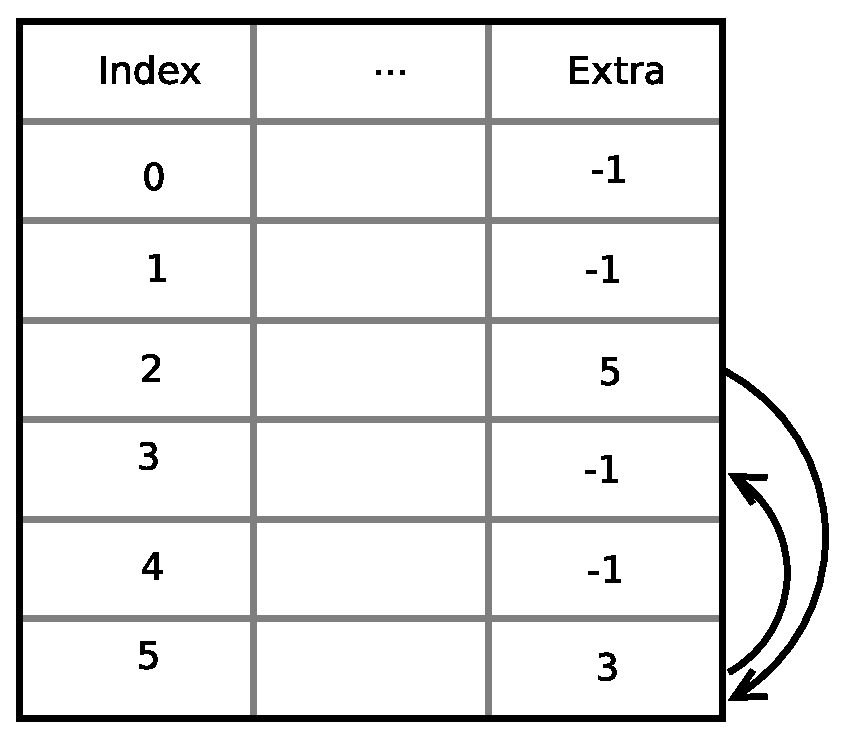
\includegraphics[width=2in,scale=0.4]{../images/diagrams/freelist4.eps}} \\
\hline
\end{tabular}
\cprotect\caption{Example illustrating the working of the freelist in the vector. \verb+_vfree+ stores the starting index of the freelist. A value of $-1$ in the extra field indicates that the entry is in use and hence not a part of the freelist. The address, gateway, mask and port fields are not shown.}
\label{fig:freelisteg}
\end{center}
\end{figure}


The use of \emph{extra} is illustrated with the help of an example in Figure \ref{fig:freelisteg} for the sample vector shown in Table \ref{tbl:vector}. From the example we can see that reads and deletions are O(1). Insertions are O(1) amortized over the cost of many insertions. This is because the vector is dynamically resized when it is full.\\

\paragraph{Dynamic resize}
The vector is initialized to hold a specific number of entries (\verb+_capacity+). The number of entries currently in use in the vector is \verb+_n+. The \verb+push_back()+ function adds an entry to the vector. This increments \verb$_n$ by one. If the vector is full (i.e.\verb+_n+ $\ge$ \verb+_capacity+), it is resized to double the value of its previous capacity with a call to \verb+reserve_and_push_back()+.

\section{The Problem}
\label{sec:problem}
Our goal is to improve lookup performance by allowing for multithread access to Click elements. In this section we look at existing problems which hinder safe multithreaded access.\\

This section is divided into Updater-Updater Conflicts and Reader-Updater Conflicts. The Updater-Updater conflicts section describes how multiple updaters can cause race conditions which corrupt the state of shared data structures. The Reader-Updater Conflicts section describes how a reader racing with an updater might read stale or invalid data.
\subsection{Updater-Updater Conflicts}
We now deal with race-conditions and conflicts arising due to multiple updaters running concurrently using the same instance of RadixIPLookup. When multiple threads use the same instance of RadixIPLookup, they access the same data structures within RadixIPLookup.
\paragraph{Radix Tree}
The radix tree suffers from Update-Update conflicts. If multiple updaters try to modify the same region of the tree, there is a race in \verb+change()+ for the assignment of the child pointer. This could cause some of the updates to be lost and also cause a memory leak. The size of the memory leak can be equal to the depth of the tree times the size of a radix node.\\

The race described above is illustrated with the help of Listing \ref{change}.
\begin{lstlisting} [label =change, caption={A snippet of the change() function where a race can cause a memory leak. This is illustrated in \ref{fig:raceinchange}},float=tph]
  int
  RadixIPLookup::Radix::change(uint32_t addr, uint32_t mask,
                                          int key, bool set)
  {
    ...
    if (mask & ((1U << _bitshift) - 1)) {
      if (!_children[i1].child
      && (_children[i1].child = make_radix(_bitshift - 4, 16)))
    ...
    ...
  }
\end{lstlisting}

\begin{figure}[tph]
\begin{center}
\begin{tabular}{|c|c|}
\hline
\textbf{Thread 1} & \textbf{Thread 2}\\
\hline
\verb$!_children[i1].child$ evaluates to true. & \verb$!_children[i1].child$ evaluates to true.\\
\hline
Calls \verb$make_radix()$. &  Calls \verb$make_radix()$.\\
\hline
\begin{tabular}{p{1.5in}}  
\raisebox{2ex - \height}{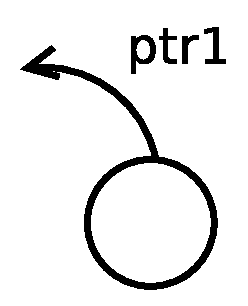
\includegraphics[scale=0.4]{../images/diagrams/radix1.eps}}\\
\verb$make_radix()$ returns pointer ptr1 to a newly created radix node.\\
\end{tabular} 
& 
\begin{tabular}{p{1.5in}}
  \raisebox{2ex - \height}{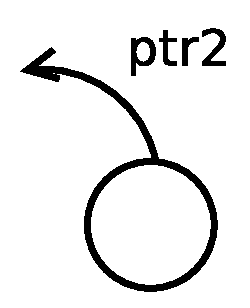
\includegraphics[scale=0.4]{../images/diagrams/radix2.eps}}\\
  \verb$make_radix()$ returns pointer ptr2  to a newly created radix node.\\
\end{tabular}\\
\hline
\begin{tabular}{p{1.8in}}  
\raisebox{2ex - \height}{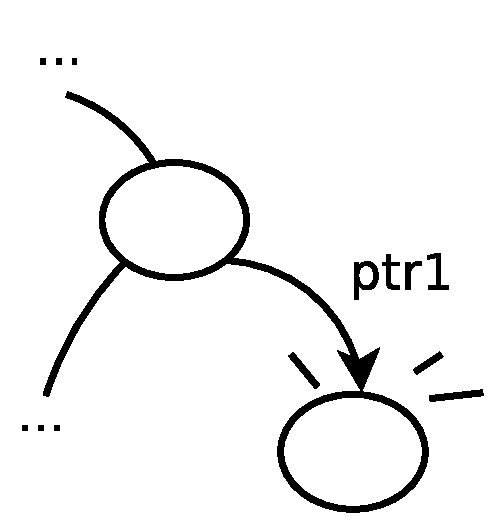
\includegraphics[scale=0.4]{../images/diagrams/radix1race.eps}}\\\\
 $\_children[i1].child = make\_radix(\_bitshift - 4, 16)$.\\
The node is added to the radix tree.\\
\end{tabular} 
& 
\begin{tabular}{p{1.8in}}
  \raisebox{2ex - \height}{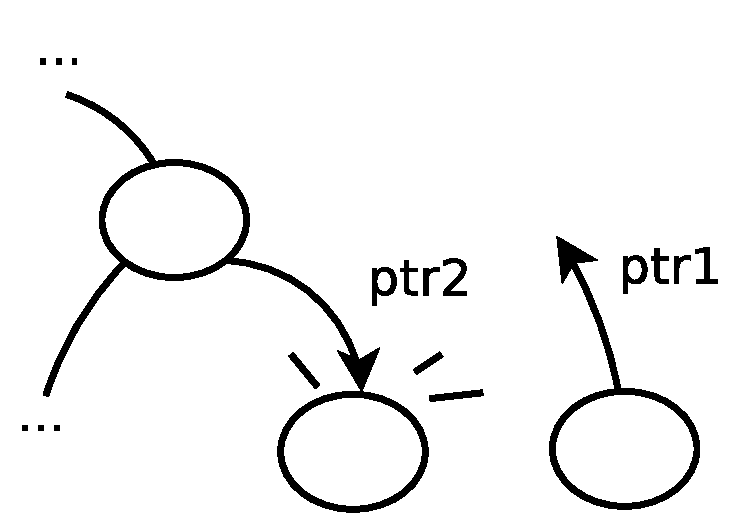
\includegraphics[scale=0.4]{../images/diagrams/radix2race.eps}}\\\\
  $\_children[i1].child = make\_radix(\_bitshift - 4, 16)$.\\
  The node is added to the tree. We have a memory leak since the older node is now orphaned. \\
\end{tabular}\\
\hline
\end{tabular}
\cprotect\caption{Example illustrating the race in the \verb$change()$ function. The \verb$change()$ function is used in the insertion of new radix nodes. Two concurrent threads insert a radix node into the tree leading to a memory leak.}
\label{fig:raceinchange}		
\end{center}
\end{figure}

The \verb+change()+ function in Listing \ref{change} is used to create a radix node for a route with a specific address, and mask. The key passed as a parameter is the index into the vector where the route is stored. Two or more concurrently executing threads create race conditions which can lead to memory leaks. This is explained pictorially in Figure \ref{fig:raceinchange}. Looking at the assignment, we see that if there are multiple threads executing \verb$change()$, there is a race for the assignment of the radix node. Multiple threads may call \verb+make_radix()+, however only one pointer which is returned by \verb+make_radix()+ is assigned. 
\paragraph{Vector}
When there are multiple updaters there is contention for acquiring an index into the vector. Many updaters trying to add a route might receive the same index value. If multiple updaters are given the same value of the index, there can be an inconsistency in the state of the vector. For example, the size of the vector might be stored wrongly or the freelist might be updated wrongly. Since the vector is resized dynamically, we could lose updates and have memory-leaks.\\

We explain the conflicts mentioned above with examples using the \verb+add_route()+ function shown in  Listing \ref{addroute}.
\begin{lstlisting}[caption = The add\_route function, label=addroute,float=tph]
  int
  RadixIPLookup::add_route(const IPRoute &route, 
                           bool set, 
                           IPRoute *old_route, 
                           ErrorHandler *)
  {
    int found = (_vfree < 0 ? _v.size() : _vfree), last_key;
    if (route.mask) {
      uint32_t addr = ntohl(route.addr.addr());
      uint32_t mask = ntohl(route.mask.addr());
      last_key = _radix->change(addr, mask, found + 1, set);
    } else {
      last_key = _default_key;
      if (!last_key || set)
      _default_key = found + 1;
    }
    if (last_key && old_route)
    *old_route = _v[last_key - 1];
    if (last_key && !set)
    return -EEXIST;
    if (found == _v.size())
    _v.push_back(route);
    else {
      _vfree = _v[found].extra;
      _v[found] = route;
    }
    _v[found].extra = -1;
    if (last_key) {
      _v[last_key - 1].extra = _vfree;
      _vfree = last_key - 1;
    }
    return 0;
  }
\end{lstlisting}
We consider two cases, one in which the concurrently executing threads retrieve an index from the freelist, the other in which the concurrently executing threads make a call to \verb+push_back()+ on the vector.

\paragraph{Case 1: Concurrent updaters use the freelist}
We now illustrate how a race condition can corrupt the state of the vector. The same example is illustrated pictorially in Figure \ref{fig:raceinfreelist}
Assume the freelist is as follows before the execution of this code sequence:\\
\verb$freelist::{ 3 -> 1-> 5, _vfree =3}$. Consider the following sequence of events:
\begin{enumerate}
\item Thread 1 calls \emph{add\_route(Y,1,NULL,NULL) Y.addr = A, Y.mask =M}.
\item Thread 2 calls \emph{add\_route(Y,1,NULL,NULL) Y.addr = A, Y.mask =M}.
\item Updater 1 and Updater 2 execute line 4 concurrently and recieve the same value of \emph{found}. Let us assume that \emph{found} is some key within the vector and is not equal to \emph{\_v.size()}. Updater 1 executes line 7 first. This updates the key in the radix tree to be the value \emph{found} which is $3$ according to our example.
\item Updater 2 executes line 7. The value of the key is set to \emph{found} which is $3$ since the freelist has not changed.
\item Updater 1 executes the remaining code in \verb+add_route()+ including line 27 which sets  \verb+_v[found].extra+ to $-1$ (which means that the index is in use). After the Updater 1 has finished executing add\_route(), the freelist reads\\
\verb$freelist::{ 1-> 5, _vfree =1}$.
\item Updater 2 executes the remaining code sequence. It executes line 24 which sets \verb+_vfree+ to \emph{\_v[found].extra}. \verb+_v[found].extra+ has been set to $-1$ by Updater 1. Thus \verb+_vfree+ is now $-1$.\\
The state of the freelist is now \verb$freelist::{ 1-> 5,_vfree = -1}$. The correct state is \verb$freelist::{ 1-> 5, _vfree = 1}$. If \verb+_vfree+ is $-1$, it means that there are no more free keys in the vector, which is not true. This sequence brings the vector into an inconsistent state.
\end{enumerate}

\begin{figure}[tph]
\begin{center}

\begin{tabular}{|p{4.6in}|}
\hline
Initial state of the freelist:\\
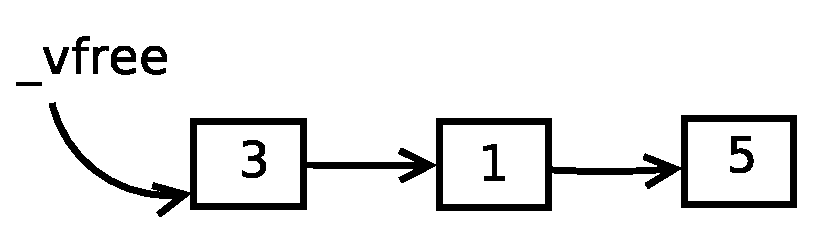
\includegraphics[scale=0.4]{../images/diagrams/freelistrace1}\\
\hline
\end{tabular}
\begin{tabular}{|p{2.2in}|p{2.2in}|}
\hline
\textbf{Thread 1} & \textbf{Thread 2}\\
\hline
calls
\begin{Verbatim}[baselinestretch=1,fontsize=\small]
add_route(X,1,NULL,NULL) 
\end{Verbatim}
&
calls
\begin{Verbatim}[baselinestretch=1,fontsize=\small]
add_route(Y,1,NULL,NULL)
\end{Verbatim}
\\
\hline
Executes:
\begin{Verbatim}[baselinestretch=1,fontsize=\small]
found= (_vfree < 0 ?
        _v.size():_vfree)
\end{Verbatim}
Obtains a value $found = \_vfree = 3$ 
&
Executes:
\begin{Verbatim}[baselinestretch=1,fontsize=\small]
found= (_vfree < 0 ?
        _v.size():_vfree)
\end{Verbatim}
Obtains a value $found = \_vfree = 3$\\
\hline
\begin{tabular}{p{1.8in}}
Executes:
...
\begin{Verbatim}[baselinestretch=1,fontsize=\small]
_v[found].extra = -1;
\end{Verbatim}
As a result, the freelist is updated as shown in the figure. \\\\
\hline
\raisebox{2ex - \height}{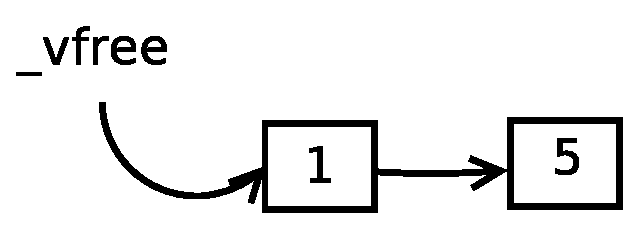
\includegraphics[scale=0.4]{../images/diagrams/freelistrace2}}\\\\
\end{tabular}
&
Thread is blocked or paused or context-switched.\\
\hline
Thread exits \verb+add_route()+.
&
\begin{tabular}{p{1.8in}}
Executes:\\
\verb$_vfree = _v[found].extra$.\\
\verb$_v[found].extra$ was set to $-1$ by thread 1. So \verb$_vfree$ is $-1$.
Freelist is now updated as shown in the figure. This is wrong since $\_vfree$ is -1 although there are unused indices in the freelist. A value of $-1$ for \_vfree indicates that the freelist is empty which is untrue.\\\\
\hline
\raisebox{2ex - \height}{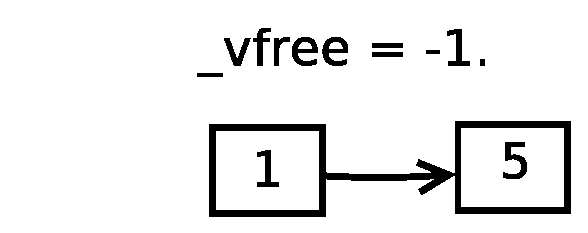
\includegraphics[scale=0.4]{../images/diagrams/freelistrace3}}\\\\
\end{tabular}\\
\hline
\end{tabular}
\cprotect\caption{The example illustrates how two concurrent updaters can corrupt the sate of the freelist if they call \verb+add_route()+. The initial state of the freelist is as shown in the figure. The first parameter is the route, the second parameter asks the function to use the route supplied even if a route previously existed for that IP Address. The third parameter \emph{old\_route} retrieves a preexisting route for that IP if it is not set to NULL. The fourth parameter is the error handler.}
\label{fig:raceinfreelist}
\end{center}		
\end{figure}

\paragraph{Case 2: Concurrent updaters call \emph{push\_back} }
Now consider the case when\\ \verb+_v.push_back()+ is executed concurrently. For this we will look at the Click code from vector.cc in Listing \ref{pushback}.
\begin{lstlisting}[caption = The push\_back() function, label=pushback]
  template <class T> inline void
  Vector<T>::push_back(const T& x)
  {
    if (_n < _capacity) {
      new(velt(_n)) T(x);
      ++_n;
    } else
    reserve_and_push_back(RESERVE_GROW, &x);
  }
\end{lstlisting}
We first consider the case when there is enough space in the vector. Updater1 and Updater2 use the same value of \verb+_n+. The updater which wins the race installs its key at position i, and the other update is lost.
We now consider the case when there is not enough space in the vector. The expression \verb$_n < _capacity$ evaluates to false. Some of the race conditions here could bring the vector to an inconsistent state or cause memory leaks. They are better understood with the help of the striking graphic example in Figure \ref{fig:raceinreserve} and the \verb+reserve_and_push_back()+ function shown in Listing \ref{reserveandpushback}. The assignment of \verb+new_l+ in line 15 of Listing \ref{reserveandpushback} is a race condition which can lead to a memory leak. The size of the leak is equal to the size of \verb+new_l+. The other consequence is that one update will be lost. If both the updaters call CLICK\_LFREE() in line 14, we could have a segmentation fault.

\begin{figure}[tph]
\begin{center}
\begin{tabular}{|c|c|}
\hline
\textbf{Thread 1} & \textbf{Thread 2}\\
\hline
Calls \verb$reserve_and_pushback()$. &  Calls \verb$reserve_and_pushback()$.\\
\hline
\begin{tabular}{p{1.5in}}
\\  
\raisebox{2ex - \height}{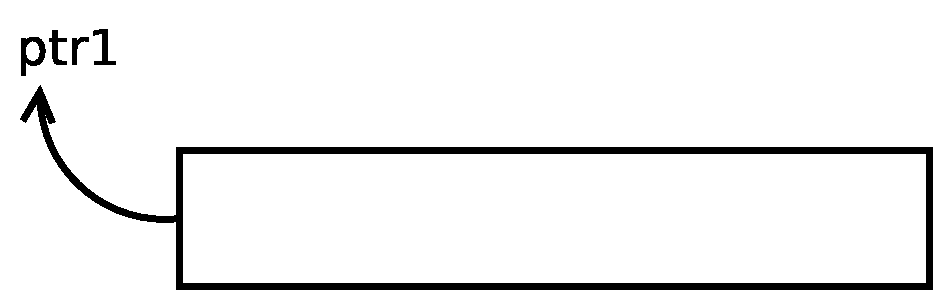
\includegraphics[scale=0.3]{../images/diagrams/vectorptr1}}\\
\verb$CLICK_LALLOC()$ returns pointer ptr1 to a newly allocated vector.\\
\end{tabular} 
& 
\begin{tabular}{p{1.5in}}
  \\
  \raisebox{2ex - \height}{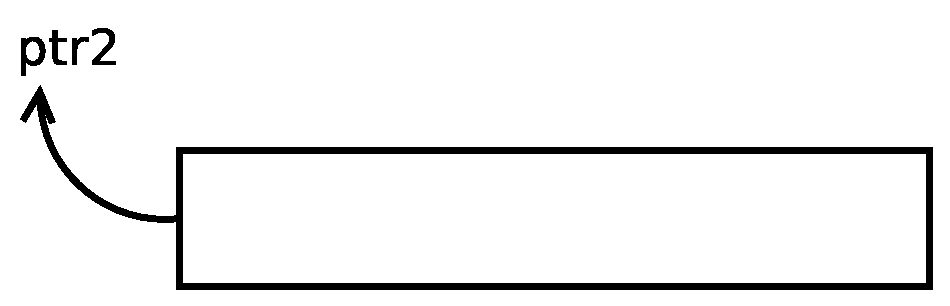
\includegraphics[scale=0.3]{../images/diagrams/vectorptr2}}\\
  \verb$CLICK_LALLOC()$ returns pointer ptr2 to a newly allocated vector.\\
\end{tabular}\\
\hline
\begin{tabular}{p{1.8in}}  
\raisebox{2ex - \height}{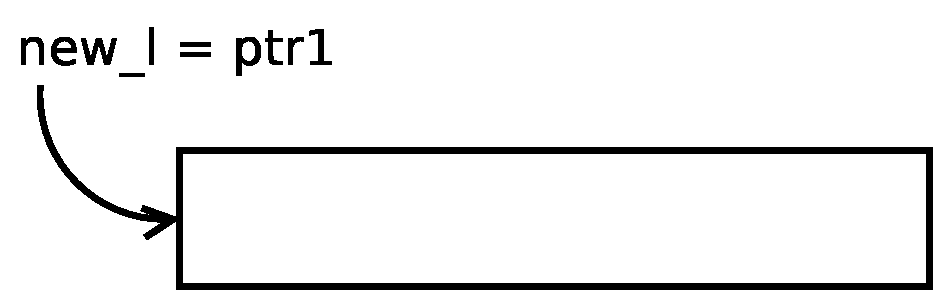
\includegraphics[scale=0.3]{../images/diagrams/vectorrace1}}\\\\
 \verb$new_l = ptr1$.\\
The node is added to the radix tree.\\
\end{tabular} 
& 
\begin{tabular}{p{1.8in}}
  \\
  \raisebox{2ex - \height}{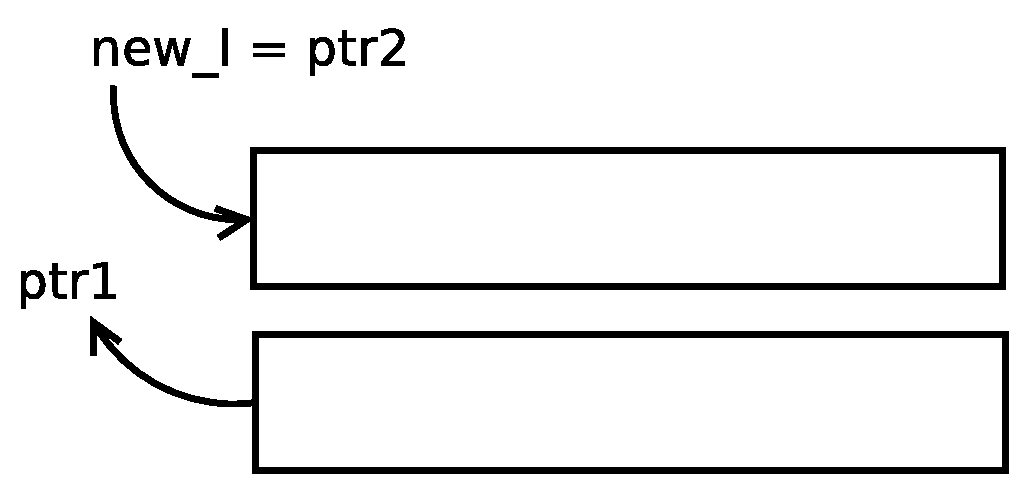
\includegraphics[scale=0.3]{../images/diagrams/vectorrace2}}\\\\
  \verb$new_l = ptr2$.\\
  We have a memory leak since the older node is now orphaned.\\
\end{tabular}\\
\hline

\begin{tabular}{p{1.8in}}  
\raisebox{2ex - \height}{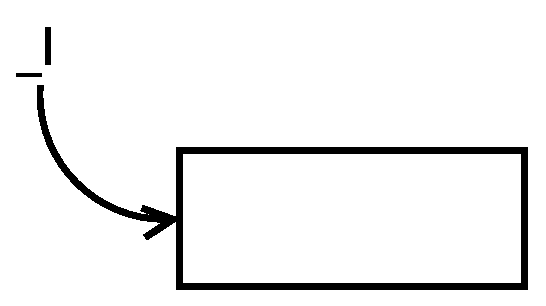
\includegraphics[scale=0.3]{../images/diagrams/vectorrace3}}\\\\
 \verb$CLICK_LFREE(_l, ...)$.\\
 The pointer to the old vector is freed.\\
  \raisebox{2ex - \height}{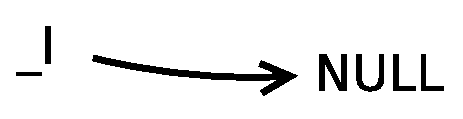
\includegraphics[scale=0.3]{../images/diagrams/vectorrace4}}\\\\
\end{tabular} 
& 
\begin{tabular}{p{1.8in}}
  \\
  \raisebox{2ex - \height}{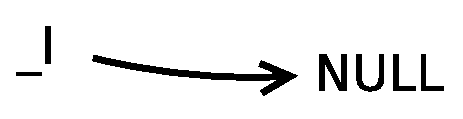
\includegraphics[scale=0.3]{../images/diagrams/vectorrace4}}\\\\
\verb$CLICK_LFREE(_l, ...)$.\\  
   \raisebox{2ex - \height}{
\includegraphics[scale=0.3]{../images/diagrams/vectorrace5}}\\\\
  We have a segmentation fault since the thread attempts to free a pointer which is already freed.\\
\end{tabular}\\
\hline
\end{tabular}
\cprotect\caption{Example illustrating the race during a dynamic resize of the vector.}
\label{fig:raceinreserve}
\end{center}		
\end{figure}


\begin{lstlisting}[caption= reserve\_and\_push\_back(), label =reserveandpushback,float=tph]
  Vector<T>::reserve_and_push_back(size_type want, 
                                  const T *push_x)
  {
    if (want < 0)
    want = (_capacity > 0 ? _capacity * 2 : 4);
    if (want > _capacity) {
      T *new_l = (T *) CLICK_LALLOC(sizeof(T) * want);
      if (!new_l)
      return false;
      for (size_type i = 0; i < _n; i++) {
        new(velt(new_l, i)) T(_l[i]);
        _l[i].~T();
      }
      CLICK_LFREE(_l, sizeof(T) * _capacity);
      _l = new_l;
      _capacity = want;
    }
    if (unlikely(push_x))
    push_back(*push_x);
    return true;
  }
\end{lstlisting}
\paragraph{Verifying conflicts in Click}
An approach similar to the one described in the Reader-Updater Conflicts section was followed here. We created a Click elements called BashRadixIPLookup and PoundRadixIPLookup which repeatedly add and delete the same route having the same address but different values of the port. Both BashRadixIPLookup and PoundRadixIPLookup run concurrently on the same instance of RadixIPLookup. This concurrency is ensured by using the \emph{StaticThreadSched()} element in the script.
\begin{code}
  BashRadixIPLookup::repeat 10,000 times {
    add_route (A,X);
    delete_route (A,X);
  }
  PoundRadixIPLookup::repeat 10,000 times {
    add_route (B, Y);
    delete_route (B,Y);
  } 
\end{code}
The tests resulted in segmentation faults and assertion failures, which did not occur if locks were acquired during updates.
\subsection{Reader-Updater Conflicts}
The conflicts in the RadixIPLookup element occur primarily in two data structures: vector used to store the routes, and the radix-tree which stores a key indexing into the vector. The sections below describe the conflicts which occur in each of these data structures.
\paragraph{Radix Tree:}
This section describes some of the reader-updater conflicts which exist and why they are not a source for concern. We take a look at a race which might arise and explain why it is not a serious problem.\\

We now look at deletion of nodes within a radix tree. All pointers to the radix node are freed during a clean up phase of RadixIPLookup before it is destroyed. When a route is removed, the radix node corresponding to the route is not freed immediately. Instead all the radix nodes in the tree are deleted together at the end. This takes place in the call to \verb+free_radix()+. \verb+free_radix()+ is called on an instance of RadixIPLookup just before the instance is destroyed.\\

We will now look at a race condition which can occur in the radix tree when a reader and an updater execute concurrently. Consider a case where we have a reader and an updater running concurrently. The updater deletes route X, the reader performs a lookup on the very route X.
\begin{figure}[tph]
\begin{center}
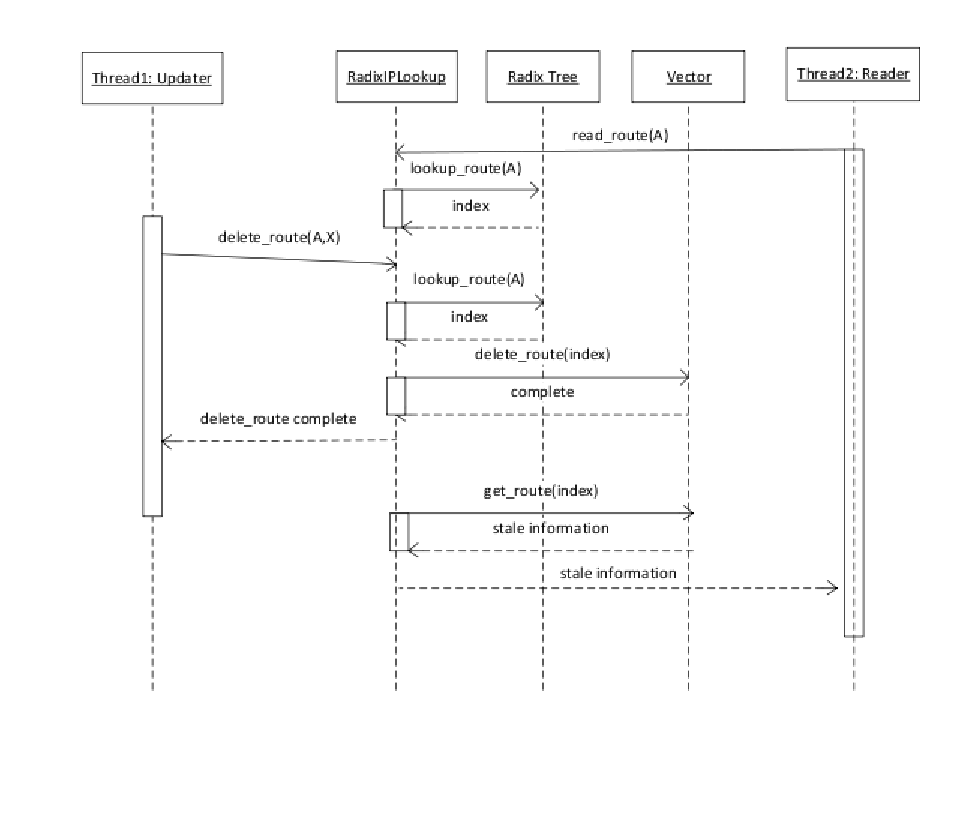
\includegraphics[scale=0.6]{../images/diagrams/race1eps.eps}
\end{center}
\caption{Race condition with a concurrent reader and updater}
\label{race1figure}
\end{figure}
\\\\
We have two threads one running: \emph{Updater:: \{remove Route X\}} and the other running: \emph{Reader::\{read Route A\}}. The reader might receive stale information for Route X. This happens if the reader acquires a reference to the radix node containing Route X before the pointer is removed from the tree. The race is illustrated with the help of the sequence diagram in \ref{race1figure}. However, readers which execute after the updater has finished will not recieve stale data for Route X.
\begin{lstlisting}[caption= The remove\_route() function, label=removeroute,float=tph]
  int
  RadixIPLookup::remove_route(const IPRoute& route, 
                              IPRoute* old_route, 
                              ErrorHandler*)
  {
    int last_key;
    if (route.mask) {
      uint32_t addr = ntohl(route.addr.addr());
      uint32_t mask = ntohl(route.mask.addr());
      // NB: this will never actually make changes
      last_key = _radix->change(addr, mask, 0, false);
    } else
    last_key = _default_key;
    if (last_key && old_route)
    *old_route = _v[last_key - 1];
    if (!last_key || !route.match(_v[last_key - 1]))
    return -ENOENT;
    _v[last_key - 1].extra = _vfree;
    _vfree = last_key - 1;
    if (route.mask) {
      uint32_t addr = ntohl(route.addr.addr());
      uint32_t mask = ntohl(route.mask.addr());
      (void) _radix->change(addr, mask, 0, true);
    } else
    _default_key = 0;
    return 0;
  }
\end{lstlisting}
The occurrence of the race mentioned above is rather rare: firstly a read intensive, infrequent update workload is expected but the aforementioned race is more likely in an update intensive workload. Secondly reads are fast compared to updates, so the possibility that a read operation starts before an update and ends after an update is quite small. That being said, we assume that the consequences of the race illustrated in the example above are acceptable. This is justified by the argument that the reader received a stale route: it was once valid route for the given address, and the ultimate price paid is the price of one wrong lookup.
\paragraph{Vector:}
The library files in Click include a generic dynamically resized Vector class. This class and its use in RadixIPLookup has been explained in the Background section. The conflicts are explained in the context of the \verb+add_route()+ function which adds a route to the radix tree. The code for the \verb+add_route()+ function is given in Listing \ref{pseudoaddroute}. The way an index is obtained for insertion is summarized in the pseudocode below. 
\begin{lstlisting}[caption = Pseudocode for acquiring an index in add\_route, label=pseudoaddroute]
  if(free_list is not empty)
  {
    index = free_list;
    free_list = free_list -> next;
    _v[free_list.index] = val;
  }
  else 
  _v.push_back(val);
\end{lstlisting}
We can observe at least two inadmissible conflicts which can be caused by race conditions. Firstly, if two updaters and a reader run concurrently, the reader might get an index into an entry which has been freed and reused. The reader may end up receiving a route which is incorrect for the IP address in question. Secondly, a reader might access invalid memory in the presence of a concurrent updater. One must recall that the \verb+push_back()+ operation dynamically resizes the vector if necessary. If an updater initiates a dynamic resize operation amidst a concurrent reader, the reader might access invalid memory.

\paragraph{Verifying conflicts in Click}
The first conflict mentioned above was verified by running Click scripts. New elements were created and run in multi-threaded mode.The \emph{StaticThreadSched()} element was used to specify the thread on which the element must be run. Listing \ref{scriptlisting} facilitates a clearer picture of the use of \emph{StaticThreadSched()} for this case.
\begin{lstlisting}[caption = Click script for verifying reader-updater conflicts, label=scriptlisting]
Idle
 -> r :: RadixIPLookup106(
                0.0.0.0/0   8.1.1.1 0,
                ) 
 -> Idle;

reader :: ReadRadixIPLookup106(r);
writer0:: BashRadixIPLookup106(r);
writer1 :: PoundRadixIPLookup106(r);

StaticThreadSched(
        reader 0,
        writer0 1,
        writer1  2);

DriverManager(stop);
\end{lstlisting}
We created a Click elements called BashRadixIPLookup and PoundRadixIPLookup which repeatedly add and delete a route having the for the same IP address but different port values.
\begin{code}
  BashRadixIPLookup::repeat 10,000 times {
    add_route (A,X);
    delete_route (A,X);
  }
  PoundRadixIPLookup::repeat 10,000 times {
    add_route (B, Y);
    delete_route (B,Y);
  } 
  ReadRadix:: repeat 10,000 times {
    port = Read (A);
  }
\end{code}
A and B are the addresses, X and Y are the values of the port. The least-common ancestor of A and B is the root node. The parameters for \emph{Add route} mentioned here are not the same as add\_route() used in \emph{RadixIPLookup}. The pseudocode presented above is simplified to illustrate the motive behind our method of verifying conflicts.
\begin{figure}[tph]
\fbox{
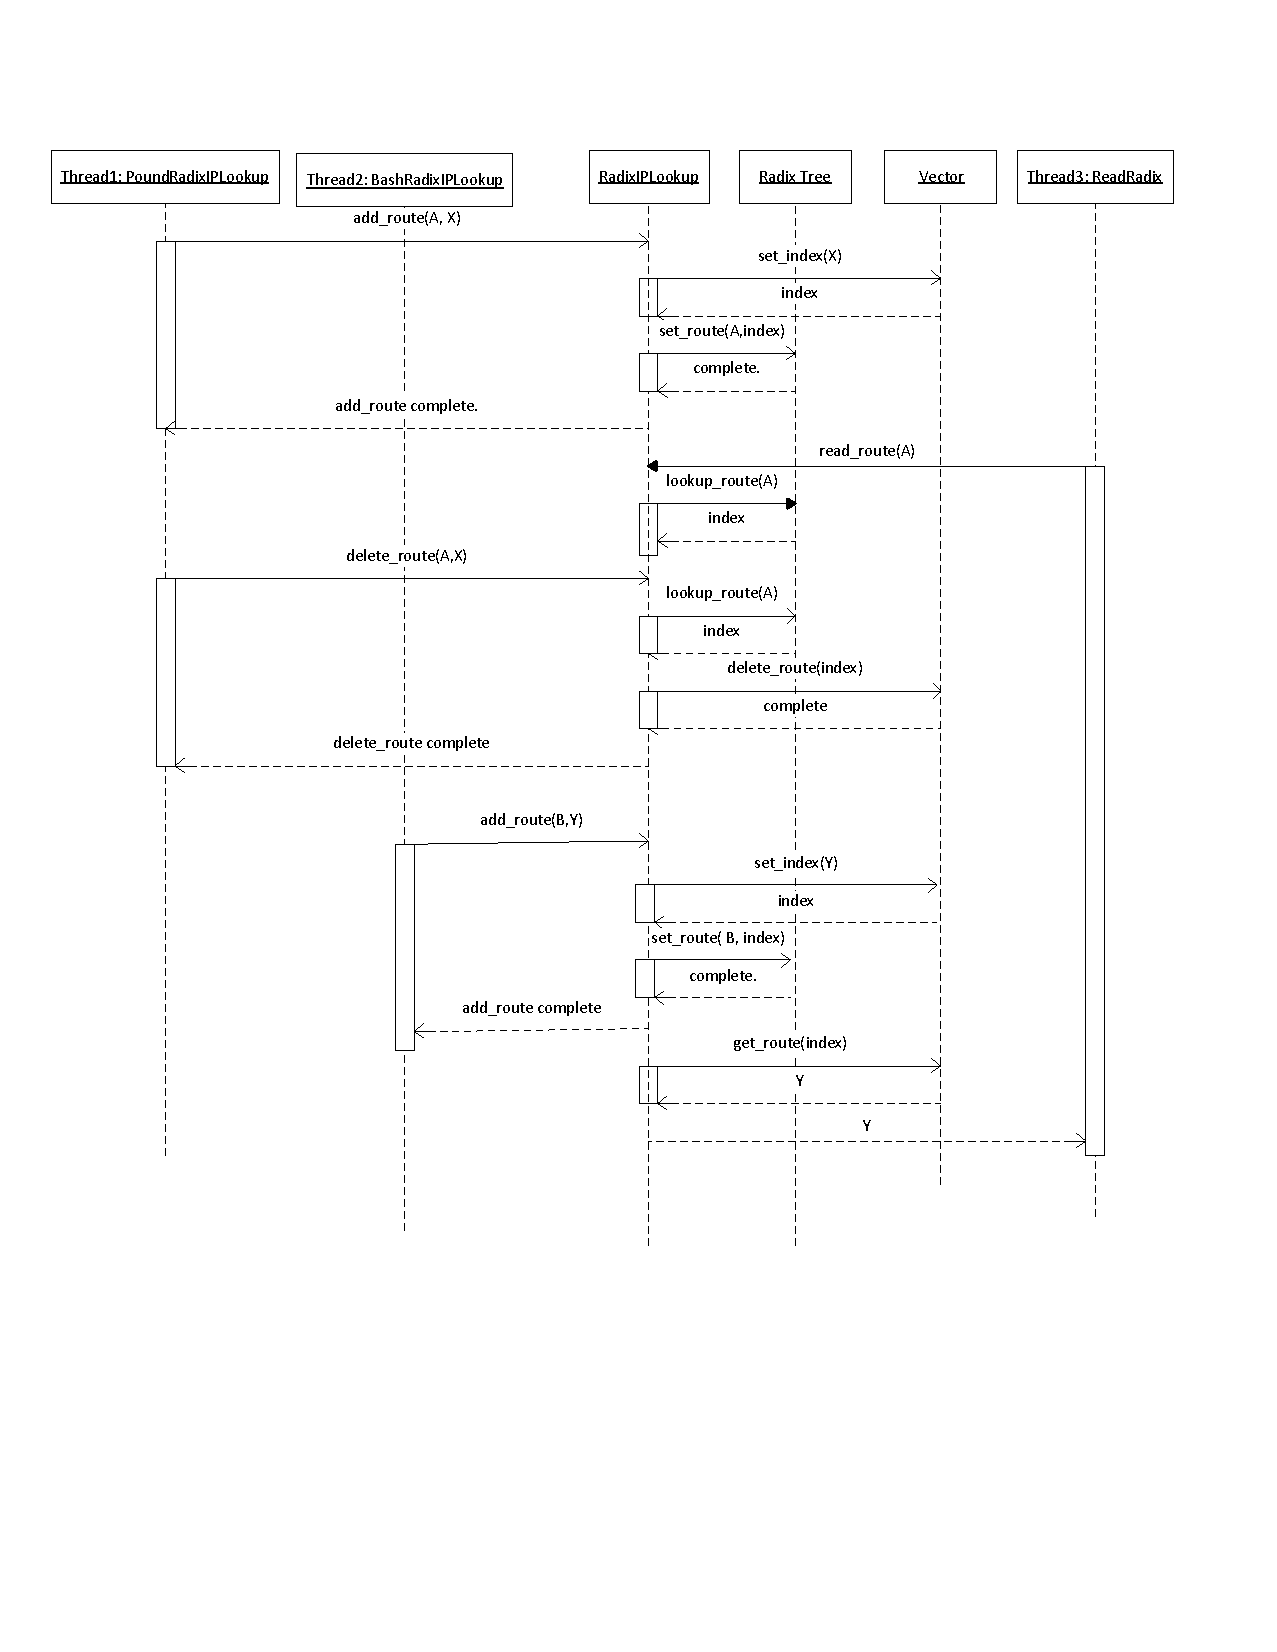
\includegraphics[scale=0.6]{../images/diagrams/race_reader.pdf}
}
\caption{Race condition with a concurrent reader and updater}
\label{race_readerfigure}
\end{figure}
\\
Locks are acquired during updates since we want to verify reader-updater conflicts as opposed to updater-updater conflicts. All three of these are run concurrently on the same instance of RadixIPLookup. The race is illustrated with the help of a sequence diagram in Figure \ref{race_readerfigure}.\\

A thread-safe implementation will have us expect that we always get X or the default route. A default route is returned if there was no prefix matching the route being looked up in the tree. But we see that the lookup sometimes returns Y which is incorrect.
\section{The Solution}
\label{sec:solution}
The race conditions described in the previous sections occur due to threads accessing shared data structures. In order to provide a thread-safe solution, several approaches were tried and their performance was compared. This section describes the different approaches tried in order to solve the problem. Coarse grained locking, fine-grained locking and Read Copy Update are the different methods we have tried. The Read Copy Update approach is the focus of this document, and a justification of its working and the implementation details are exposed in Section \ref{sec:rcu}.
\subsection{Reader-Writer Lock}
Locking solves our problems since it prevents two threads from simultaneously accessing shared data. We chose a reader-writer lock, since the typical workload for a router is read intensive with few updates. In the absence of an updater, all readers can access shared data without contending for the lock. 
 Our coarse-grained locking approach involves locking around the entire read-side or update-side critical sections. This is illustrated in the \verb+add_route()+ function shown in Listing \ref{addroutereaderwriterlocklisting}, where a lock is acquired around the entire update-side critical section. Similar locking is used around the read-side critical section in \verb+lookup_route()+ (Listing \ref{lookuproutereaderwriterlocklisting}).
\begin{lstlisting}[caption = Reader-writer lock usage in lookup\_route(), label=lookuproutereaderwriterlocklisting,float=tph]
int RadixIPLookup107::lookup_route(IPAddress addr, 
                                   IPAddress &gw) const
{  
    _lock.acquire_read();
    ...
    read side critical section
    ...
    _lock.release_read();
    return port;
}
\end{lstlisting}
\begin{lstlisting}[caption = Reader-writer lock usage in add\_route(), label=addroutereaderwriterlocklisting,float=tph]
int
RadixIPLookup107::add_route(const IPRoute &route, 
                            bool set, 
                            IPRoute *old_route, 
                            ErrorHandler *)
{
  _lock.acquire_write();
  ...
  write-side crtical section
  ...
  _lock.release_write();
  return 0;
}
\end{lstlisting}
\pagebreak
\subsection{Read Copy Update}

\label{sec:rcu}
Coarse and fine-grained locking solve the problems we have identified, but the locking system is still over 14 times slower in a pure reader workload (See Table \ref{tbl:macro_vr_0w} for details). Our goal is to develop a solution with very low read side overhead, so we turn to Read-Copy-Update.\\

Quiescent State Based Reclamation (QSBR) is an approach with optimal performance at the cost of a more constrained application design\cite{hart}. Using QSBR requires that we identify \emph{grace periods}. A grace period is a state in which each thread has undergone at least one \emph{quiescent state}. A quiescent state is a state where a thread does not have any references to mutable data structures. This could be an idle-loop or a state where the thread is running code which does not access any shared data.\\

RCU allows readers to proceed concurrently with an updater. The updater can \textbf{remove} shared data structures, but is not allowed to \textbf{delete} it. Multiple copies of shared data structures are maintained. The old copies are deleted when they are no longer being used. A grace period for a certain copy of a shared data structure is a period where we can safely delete it. Figure \ref{fig:rcuexp1} illustrates this concept.

\begin{figure}[float=tph]
\begin{center}
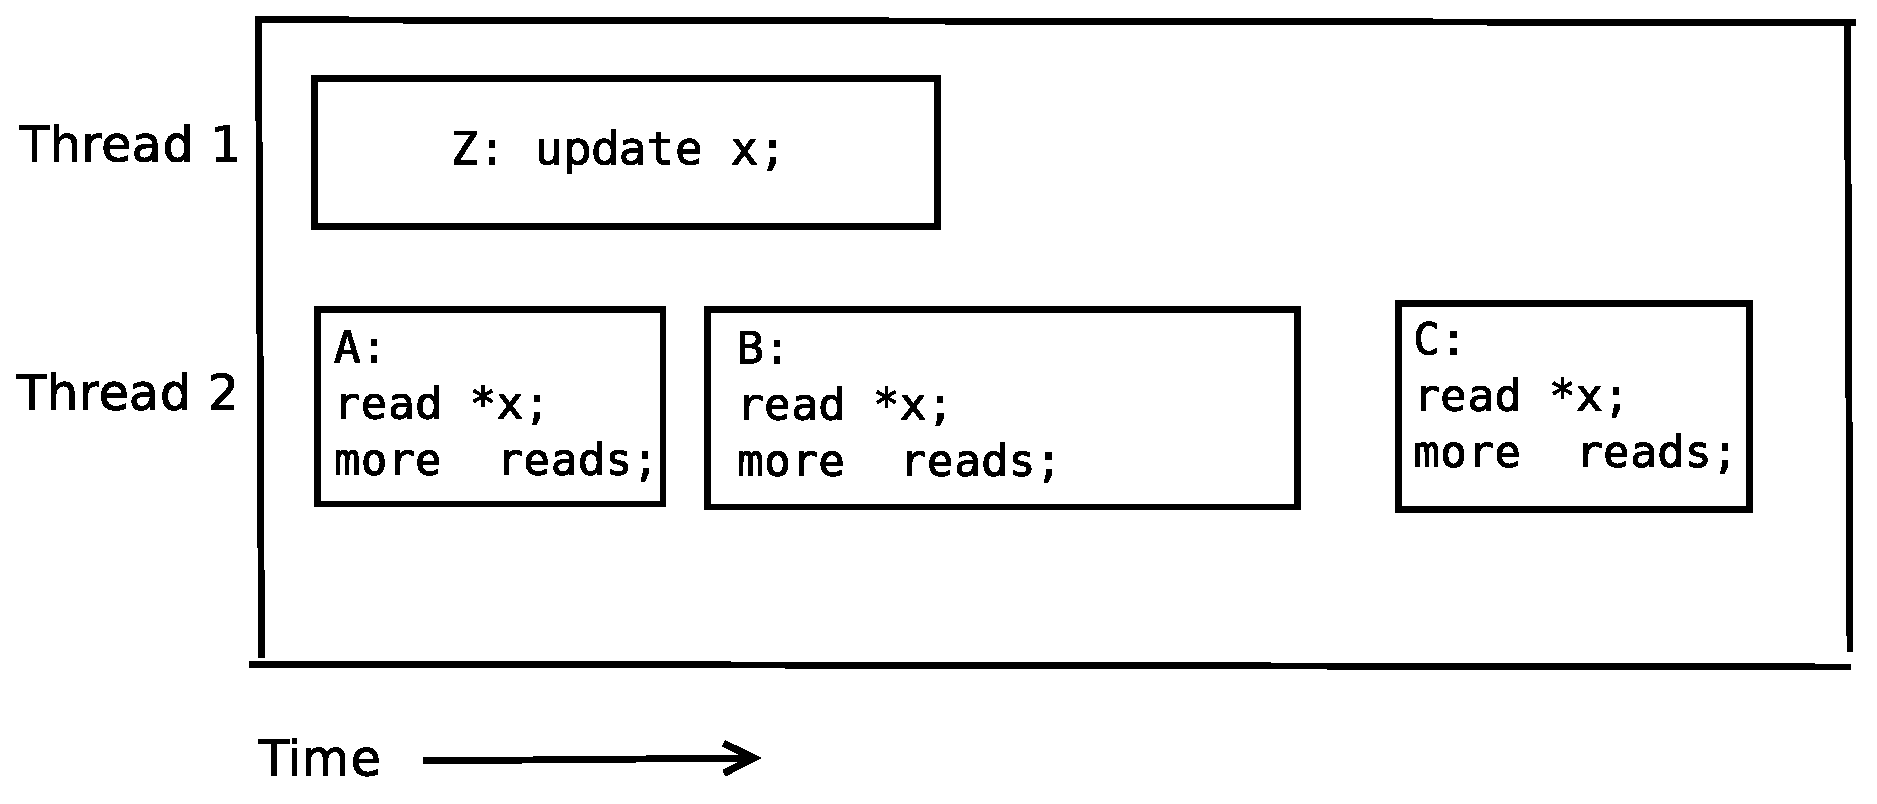
\includegraphics[scale=0.4]{../images/diagrams/rcuexp0}
\caption{Thread 1 and Thread 2 begin concurrent execution. A,B and C represent read-side critical sections which read the pointer \emph{x}. Z is an update-side critical section which updates the pointer \emph{x} by deleting the old pointer. A and B access \emph{x} when Z is in progress. We allow Z to remove the old pointer but we do not allow Z to \textbf{free} it. C reads the value of \emph{x} \textbf{after} Task Z has finished; it is not dependent on the older value of \emph{x}. It is safe to delete the older copy of \emph{x} after A and B have completed.}
\label{fig:rcuexp1} 
\end{center}
\end{figure}

The subsequent sections explain how we locate quiescent states and grace periods in Click.
\subsubsection{RCU Using Timers}
\label{sec:rcutimers}
IP lookups are read-side critical sections. An IP lookup reads the routing table which is a shared data structure. IP lookups using RadixIPLookup finish within $1000 ns$ on modern commodity machines \cite{lookuptime}. A fixed time interval $\ge 1000 ns$ can be a grace period to free stale data-structures. An interval of $1000 ns$ leads to very frequent reclamations. A very wide time interval can lead to a infrequent reclamations and a large memory footprint. So a convenient interval of $500ms$ is chosen.\\ 

Figure \ref{fig:rcutimer} explains the working of the timer mechanism. Our implementation involved using the Click Timer class to schedule reclamations. Click provides a Timer class which runs call-back functions at specified time-intervals. We use this to schedule a callback which reclaims freed data at a time interval of $500 ms$.
\begin{figure}[float=tph]
\begin{center}
\includegraphics[scale=0.28]{../images/diagrams/rcutimer}
\caption{ Three threads run concurrently. In the first 500 ms interval, an updater changes a shared data structure. Readers which have started before the update completes recieve the older value of \emph{x}. Readers which begin after the updater completes recieve the newer value. In each interval, stale data from the intervals prior to the previous interval can be reclaimed. It is safe to reclaim \emph{x} during or after the third interval and safe to reclaim \emph{y} during or after the fourth interval.
}
\label{fig:rcutimer}
\end{center}
\end{figure}

\subsubsection{RCU using the Click Scheduling Loop}
\label{rcuschedloop}

The timer expiry as a quiescent state described in Section \ref{sec:rcutimers} works well for RadixIPLookup since each lookup completes within a fixed time interval. For other elements in Click, it may not be possible to determine the duration of a read-side critical section. We wish to detect quiescent states for all other userlevel elements without having to know how long it takes for a reader task to complete. The scheme described here does not require that the reader task be of a specific duration. It does require that the reader task eventually terminate. The approach involves using the scheduling loop in Click to detect quiescent states. 

\paragraph{The Click RouterThread driver loop}
A \emph{task} in Click is something that requires CPU time or packet processing time. A task can involve performing an IP lookup, encapsulating a packet etc. Click has a class called \emph{RouterThread} which is responsible for running tasks. When Click is allowed to run with say $N$ threads, $N$ instances of \emph{RouterThread} are created. Each \emph{RouterThread} instance runs a \verb+driver()+ function which runs tasks scheduled by Click elements in a loop. We will refer to this loop as the ``driver loop''. After running a specified number of tasks, control returns to the driver loop. A highly abridged version of the driver loop is shown in Algorithm \ref{alg:driverloop}.


\begin{algorithm}[float=tph]
\begin{algorithmic}
{
\STATE $forall \mbox{ threads }t_i:$
\WHILE {$\exists \mbox{ a task for thread }t_i$} 
\STATE Run a task.
\ENDWHILE
}
\caption{The RouterThread Driver Loop}
\label{alg:driverloop}
\end{algorithmic}
\end{algorithm}

\paragraph{Grace Periods and Reclamation}
We describe our approach with the help of Figure \ref{fig:rcuexp2} in more formal terms as shown in Algorithm \ref{alg:rcu}. Each RouterThread instance maintains a local epoch counter. The local epoch counter can either be zero or one. The application has a global epoch counter. The global epoch counter is not physically stored; we only use it to explain and justify our approach. Initially all local epoch counters are set to one. After a thread completes a task, it resets its local epoch number. When the local epoch counters of all threads are reset, we reach a grace period. (All threads have released references to shared data structures they once held.) At this point, we reclaim stale data structures from the penultimate global epoch, increment the global epoch counter, set all local epoch counters and continue.
\begin{figure}[float=tph]
\begin{center}
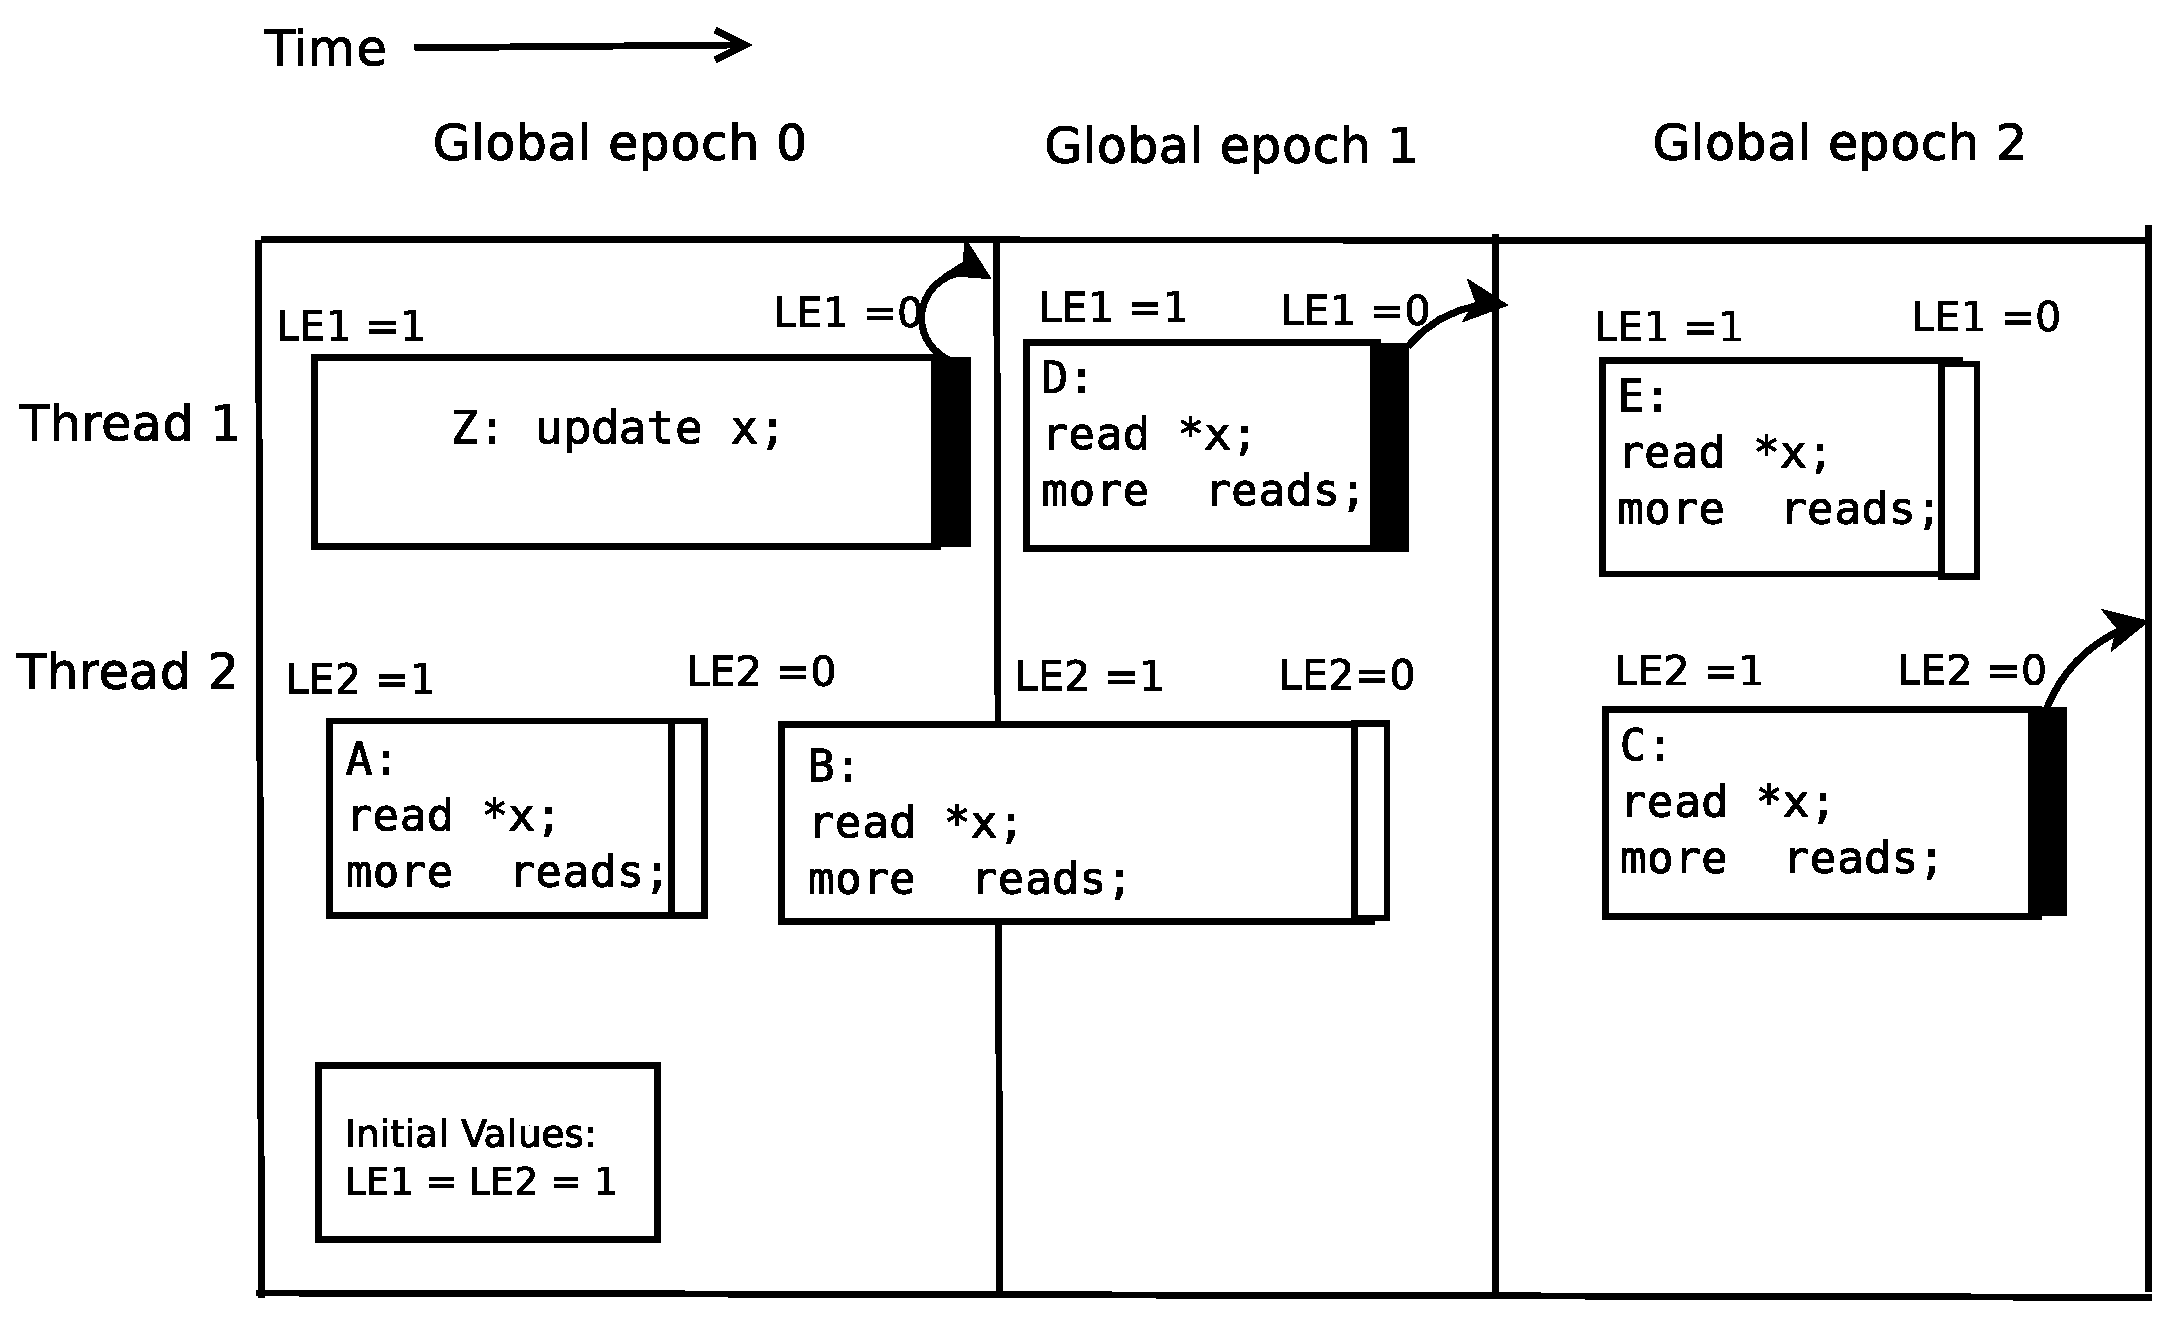
\includegraphics[scale=0.36]{../images/diagrams/rcuexp2}
\caption{Thread 1 and Thread 2 execute concurrently. 
The black rectangle indicates that a thread has updated its epoch variable and attempted to reclaim but was unsuccessful. The white rectangle indicates that a thread has updated its epoch counter and has reclaimed successfully. Following a reclamation, all local epoch counters are reset to 1. 
It is only safe to free \emph{x}  \textbf{after} \emph{global epoch 1} has passed. Task Z of \emph{Thread1} modifies the pointer \emph{x} in \emph{global epoch 0}. Task A and B dereference \emph{x} during \emph{global epochs 0} and \emph{1}. For this reason it is not safe to free \emph{x} in \emph{global epoch 0} or \emph{1}. Task C reads \emph{x} in \emph{global epoch 2}, \textbf{after} the updater has finished. For this reason, it receives the value of \emph{x} updated by task Z. We advance the \emph{global epoch counter} when we reach a grace period, i.e. when all threads cease to hold references to shared data structures.}
\label{fig:rcuexp2}
\end{center}
\end{figure}

\begin{algorithm}[float=tph]
\begin{algorithmic}
{
\STATE Each thread $t_i$ has a local epoch number $le_i$.
\STATE The application has a global epoch number $GE$.\\
\STATE Initially  $GE=0$ and $\forall t_i, le_i=1$. \\
\STATE $forall \mbox{ threads }t_i:$
\WHILE {$\exists \mbox{ a task for thread }t_i$} 
\STATE Run a task.
\STATE set local epoch  $le_i=0$.
\IF {$\forall t_i, le_i=0$}
  \STATE Reclaim stale data from $GE-2$.
  \STATE Set $GE=GE+1$.
  \STATE $\forall t_i$,Set $le_i=1$.
\ENDIF
\ENDWHILE
}
\caption{Algorithm for detecting grace periods.}
\label{alg:rcu}
\end{algorithmic}
\end{algorithm}
The transition between \emph{global epoch 1} and \emph{global epoch 2} in Figure \ref{fig:rcuexp2} is a grace period for updaters which finish in \emph{global epoch 1}. This is because any readers which start in \emph{global epoch 0} have finished by the end of \emph{global epoch 1}. It is safe to reclaim memory in \emph{global epoch 2}. We can extend this observation using Figure \ref{alg:rcu} and say that stale data accumulated in \emph{epoch N} can be reclaimed \textbf{during} \emph{global epoch N+2}. Note that we cannot do this \textbf{during} \emph{global epoch N+1} since a reader which starts in \emph{global epoch N} might not finish until the end of \emph{global epoch N+1}.\\

In order to facilitate reclamation of stale data of \emph{global epoch N-2} in \emph{global epoch N}, we maintain two lists: a \emph{reclaim\_now} list and a \emph{reclaim\_later} list. When an updater modifies a shared data structure, we maintain the older copy. The older copy is also added to the \emph{reclaim\_later} list. Whenever a grace period is reached:
\begin{enumerate}
\item Reclaim everything in the \emph{reclaim\_now} list. The \emph{reclaim\_now} list becomes empty after this step completes.
\item Swap the \emph{reclaim\_now} list and the \emph{reclaim\_later} list.\\
The \emph{reclaim\_later} list becomes empty and the \emph{reclaim\_now} list has the contents of the previous \emph{reclaim\_later} list after this step completes.
\end{enumerate}

\paragraph{RCU guarantees} 
For our scheme, we can provide the two RCU guarantees expressed in \cite{urcu}. The \emph{Grace Period Guarantee} says that a given read-side critical section cannot extend beyond both sides of a grace period. The \emph{Publication Guarantee} says that readers will see consistent newer versions of the data structures updated by writers. These guarantees are important since they show that readers always access consistent copies of data structures. 
\begin{enumerate}
\item \emph{Grace-Period Guarantee:} This guarantee states that a given read-side critical section cannot extend beyond both sides of a grace period. We now show that we can maintain this as an invariant in our scheme.

\begin{algorithmic}
\STATE Any outstanding tasks in $GE=N-2$ have finished in epoch $GE=N$.
\STATE Proof by case analysis:
\STATE Case Epoch $GE=0$: no tasks have run earlier and there have been no grace periods.
\STATE Case Epoch $GE=k$: Any outstanding tasks in $GE=k-2$ have finished and this epoch is a grace period for epoch $GE=k-2$. 
\STATE Assume that this statement is false, i.e that currently $GE=k$ and that outstanding tasks from epoch $GE=k-2$ have not finished. The condition for GE to advance to epoch $k$ from epoch $k-1$ was that all threads have their  $le_i=0$. We know that $\forall le_i, le_i=1$ at the start of epoch $k-1$. \\So $\forall \mbox{ threads }t_i\mbox{ }$ $\exists$ some task which was finished by the thread before the end of epoch $k-1$. Proved by contradiction.  
\end{algorithmic}

\item \emph{Publication Guarantee:} 
Although readers proceed concurrently with writers, readers must see either the old version of the data or the newer version. Readers should not see an inconsistent state of the data structure. Readers which begin after an updater has completed should see the newer version. In order to ensure that readers do not see an inconsistent version for RadixIPLookup, we use the bucketvector described in Section \ref{sec:finegrainedlocking}. Variables which reflect the state of the vector such as \verb+_capacity+ and \verb+_n+ are updated only after the pointers are updated. Memory barriers are also used to ensure that these variables reflect their newer values only after memory has been allocated.\\
\end{enumerate}


We observe that our approach is similar to the \emph{fuzzy barrier} approach described by Hart et al. \cite{hart}. In our scheme, the barrier is the condition which checks that all local epoch variables are set to zero. The barrier protects access to the reclamation code. This barrier is fuzzy because the threads resume execution of other tasks if they are unable cross the barrier and reclaim (non-blocking).\\
  
\subsection{Performance Hypothesis}
\label{sec:perfhypothesis}
RCU is known to work best for a reader-heavy workload with a small number of updaters. Our claim is that the RCU mechanism for click outlined above has almost zero reader-side overhead. Readers being lock-free and wait-free, we expect RCU performance to be comparable to the original version when there are only readers.\\

Updaters acquire a lock, so there is some performance penalty in the presence of updaters. We expect the RCU performance for an update-intensive workload to be comparable to that of a Reader-Writer lock.

\section{Performance Evaluation}
\label{sec:perfeval}
\subsection{Experimental Setup}
We analyzed the performance of our solutions on a Mac machine with 8 cores whose configuration is shown in Table \ref{tbl:machinemac}.
We used the CPU time reported by system utility \emph{/usr/bin/time} to measure performance.

Macrobenchmarks in Section \ref{sec:macrobenchmarks} evaluate the performance of RCU over a routing table consisting of roughly 167,000 routes. Microbenchmarks in Section \ref{sec:microbenchmarks} evaluate the performance of RCU with a over a small range of IP addresses.

\begin{table}
\begin{center}
\begin{tabular}{|l|l|l|l|l|l|}
\hline Feature & Value\\
\hline CPU &Intel(R) Core(TM) i7-2600 CPU @ 3.40GHz\\
\hline Number of Cores & 8\\
\hline Operating System & Mac OS X 10.7.2 11C74\\
\hline Cache-line size & 64 bytes\\
\hline L1 cache size (per-CPU) & 32 KB\\
\hline L2 cache size (shared by 2 CPUs) & 256 KB\\
\hline L3 cache size (shared by 8 CPUs)& 8 MB\\
\hline Main memory size & 16 GB\\
\hline
\end{tabular}
\end{center}
\caption{Machine configuration.}
\label{tbl:machinemac}
\end{table}

%% Macro benchmark sub-section
\subsection{Macro-benchmarks}
\label{sec:macrobenchmarks}

The macrobenchmarks are designed to reflect a typical software router
use case. Usually a router will encounter far more read requests (IP
lookups) as compared to write requests (routing table updates) . To
model this we consider pure reader workloads and workloads which are
read intensive with a very low fraction of writes.\\

We used a realistic routing table derived from the routeviews.org
database\cite{routeviews}. This table consists of 167,000 routes. We call this table
the \emph{167k table}. The input set was generated randomly using the
167k router configuration. A reader task consisted of performing
lookups for 100,000 inputs from this input set. An updater task
involves replacing routes for 1000 routes in the input set. Each of
the reader and updater threads execute 128 such tasks in a single run
of the test.\\

The benchmarks involving only readers were run on the RCU version,
the reader-writer lock version and the vanilla version with no
locks. When there are updaters involved in the workload the benchmark
was run on the RCU version and the reader-writer lock version. We
cannot run the workload with writers on the vanilla version since it
is not thread safe.

\subsubsection{Pure Reader Workload}
 We first look at a workload consisting of only readers. The results
 are shown in Figure \ref{img:macro_vr_0w} and Table
 \ref{tbl:macro_vr_0w}.

\begin{table}[tph]
\begin{center}
\begin{table}[tph]
\begin{center}
\begin{tabular}{|l|l|l|l|}
\hline Workload &Reader-Writer Lock (s) & RCU (s) \\
\hline  reader(s)cu & 2.915 & 1.610\\
\hline  reader(s)cu & 4.425 & 1.600\\
\hline  reader(s)cu & 6.900 & 1.660\\
\hline  reader(s)cu & 11.737 & 1.750\\
\hline  reader(s)cu & 14.387 & 1.790\\
\hline  reader(s)cu & 18.160 & 1.860\\
\hline  reader(s)cu & 22.242 & 2.450\\
\hline
\end{tabular}
\end{center}
\label{tbl:writeintensive}
\caption{Performance comparison over a pure reader workload}
\end{table}

\end{center}
\caption{Performance comparison over a workload with increasing number of readers using the 167k routing table. The first three columns show time in seconds.}
\label{tbl:macro_vr_0w}
\end{table}

\begin{figure}[tph]
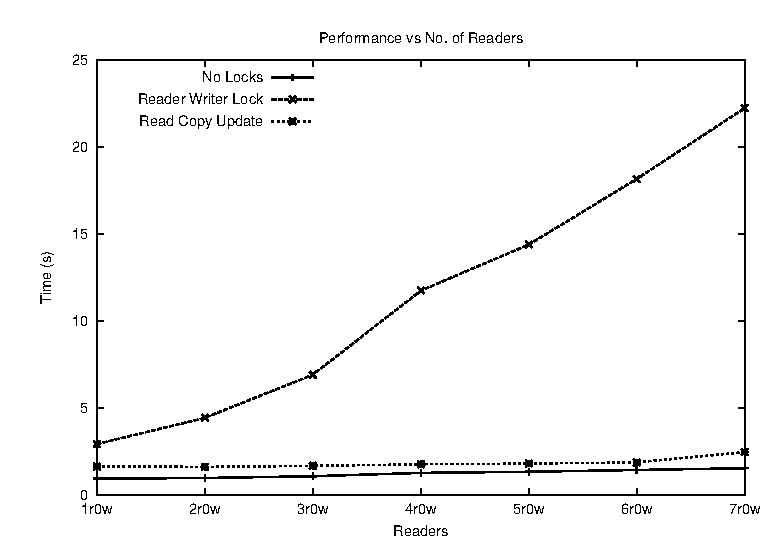
\includegraphics[scale = 0.7]{../images/graphs/macro_vr_0w}
\caption{Performance of increasing number of readers with zero writers using the 167k routing table.}
\label{img:macro_vr_0w}
\end{figure}

\begin{figure}[tph]
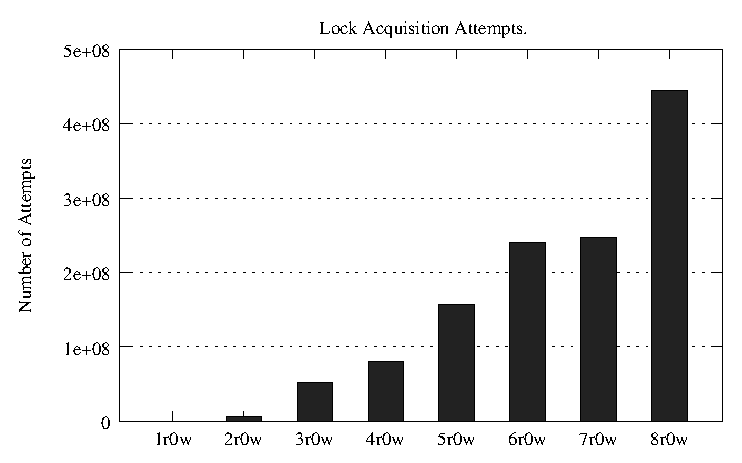
\includegraphics[scale = 0.7]{../images/graphs/profile_lockcount_macro_rwl_vr_0w}
\caption{Number of lock acquisition attempts while using the reader-writer lock for a pure reader workload.}
\label{img:profile_rwl_locks_vr_0w}
\end{figure}

From Figure \ref{img:macro_vr_0w}, we see that RCU scales much better
than the reader-writer lock version. RCU is always within $1.1$ times
the vanilla version. Time taken by the reader-writer lock increases
linearly and is up to $22$ times slower than the version without
locks.

These results validate our claim that RCU is wait-free and lock-free
for readers. In the RCU version readers do not create any
synchronization overhead. Readers in the reader-writer lock version
update a shared lock variable before they access the routing
table. The state of the shared variable needs to be updated through
all cores. As the number of threads increases, the contention causes
cache line bouncing and increased usage of the processor bus
bandwidth. For the reader-writer lock, the number of lock acquisition attempts to enter
the read side critical section is shown in Figure \ref{img:profile_rwl_locks_vr_0w}. The graph shows an increasing number of attempts for the lock with an increase in the number of threads. We can therefore attribute the  linear increase in time as the number of readers increase to the lock contention. 

\subsubsection{Read Intensive Workload With One Writer}
\begin{table}[tph]
\begin{center}
\begin{tabular}{|l|l|l|l|l|}
\hline Workload &Reader-Writer Lock (s) & RCU (s) & $\frac{\mbox{Reader-Writer Lock}}{\mbox{RCU}} $ \\
\hline 1 reader 1 writer & 2.268 & 1.550&1.463\\
\hline 2 readers 1 writer & 3.022 & 1.575&1.919\\
\hline 3 readers 1 writer & 7.683 & 1.595&4.817\\
\hline 4 readers 1 writer & 10.388 & 1.712&6.066\\
\hline 5 readers 1 writer & 13.960 & 1.785&7.821\\
\hline 6 readers 1 writer & 17.980 & 1.917&9.377\\
\hline 7 readers 1 writer & 22.443 & 2.380&9.430\\
\hline
\end{tabular}

\end{center}
\caption{Performance comparison of increasing number of readers and one writer with the 167k routing table.}
\label{tbl:macro_vr_1w}
\end{table}


\begin{figure}[tph]
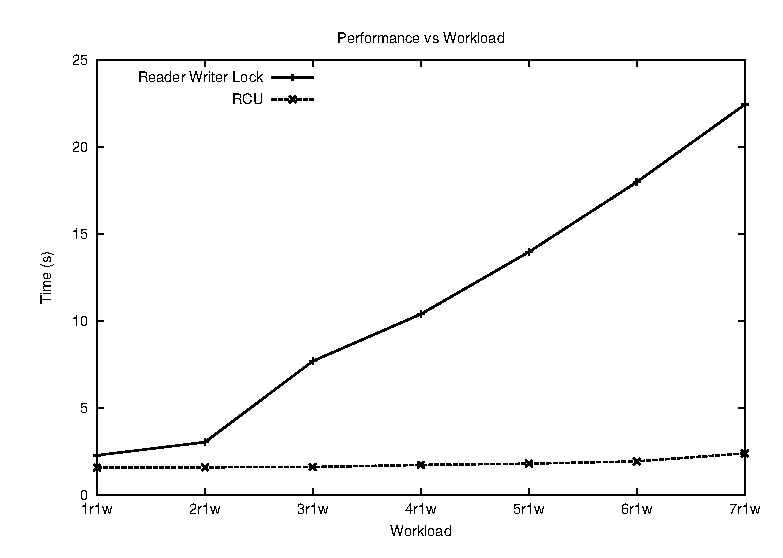
\includegraphics[scale = 0.7]{../images/graphs/macro_vr_1w}
\caption{Performance of increasing number of readers and one writer with the 167k routing table.}
\label{img:macro_vr_1w}
\end{figure}


\begin{figure}[tph]
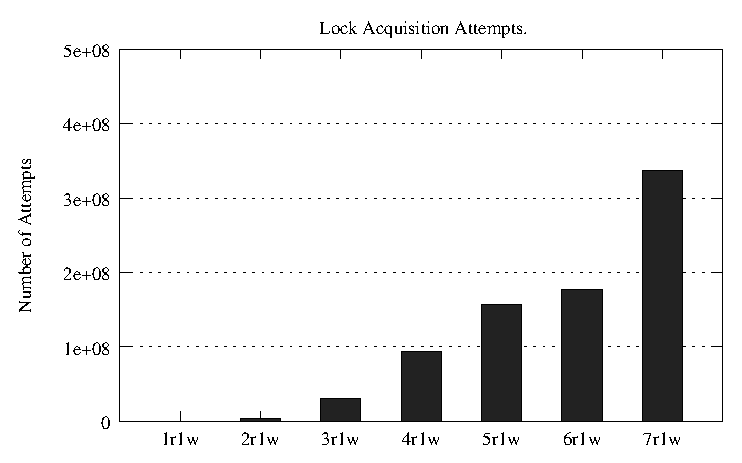
\includegraphics[scale = 0.7]{../images/graphs/profile_lockcount_macro_rwl_vr_1w}
\caption{Number of lock acquisition attempts for workload with increasing number of readers and one writer while using a reader-writer lock.}
\label{img:profile_rwl_locks_vr_1w}
\end{figure}

We also conducted a benchmark which consisted of one updater and an
increasing number of readers. The results are shown in Figure
\ref{img:macro_vr_1w} and Table \ref{tbl:macro_vr_1w}.

We see from Figure \ref{img:macro_vr_1w} that RCU scales far better
than the reader-writer lock. Time taken by the reader-writer lock
increases linearly with the number of threads. The reader-writer lock
version is over nine times slower than the RCU version for the
workload consisting of 7 readers and 1 writer. Figure \ref{img:profile_rwl_locks_vr_1w} shows the number of lock acquisition attempts while using the reader-writer lock on this workload. We can attribute the linear increase in time to the increasing lock contention. RCU does not acquire any locks in this workload. We can clearly see that RCU
outperforms the reader-writer lock for a read intensive workload with some writers.

\subsubsection{Write Intensive Workloads}
We have seen that RCU outperforms the Reader-Writer lock for reader heavy workloads. For completeness, we look at some workloads which are not common for a router: writer heavy workloads. The performance of a workload with zero readers and increasing number of writers is shown in  Figure \ref{img:macro_0r_vw} and Table \ref{tbl:macro_0r_vw}. Here, we see that the Reader-Writer Lock outperforms RCU by a factor of 1.46. We attribute this to the increased memory footprint and increased overhead in management of the reclaim lists. **Justify.

The performance of a workload consisting of one reader and increasing number of writers is shown in  Figure \ref{img:macro_1r_vw} and Table \ref{tbl:macro_1r_vw}. Although RCU does not scale, we see that it performs better than the Reader-Writer Lock.

It is clear that RCU is not as fabulous for write intensive workloads. These workloads are very uncommon for a typical router and we can accept this behavior.
 
\begin{table}[tph]
\begin{center}
\begin{tabular}{|l|l|l|l|l|}
\hline Workload &Reader-Writer Lock (s) & RCU (s) & $\frac{\mbox{Reader-Writer Lock}}{\mbox{RCU}} $ \\
\hline 0 readers 1 writer & 0.180 & 0.182&0.986\\
\hline 0 readers 2 writers & 0.203 & 0.225&0.900\\
\hline 0 readers 3 writers & 0.230 & 0.295&0.780\\
\hline 0 readers 4 writers & 0.258 & 0.362&0.710\\
\hline 0 readers 5 writers & 0.307 & 0.435&0.707\\
\hline 0 readers 6 writers & 0.352 & 0.502&0.701\\
\hline 0 readers 7 writers & 0.407 & 0.588&0.694\\
\hline 0 readers 8 writers & 0.453 & 0.660&0.686\\
\hline
\end{tabular}

\end{center}
\caption{Performance comparison of increasing number of writers and zero readers using the 167k routing table.}
\label{tbl:macro_0r_vw}
\end{table}


\begin{figure}[tph]
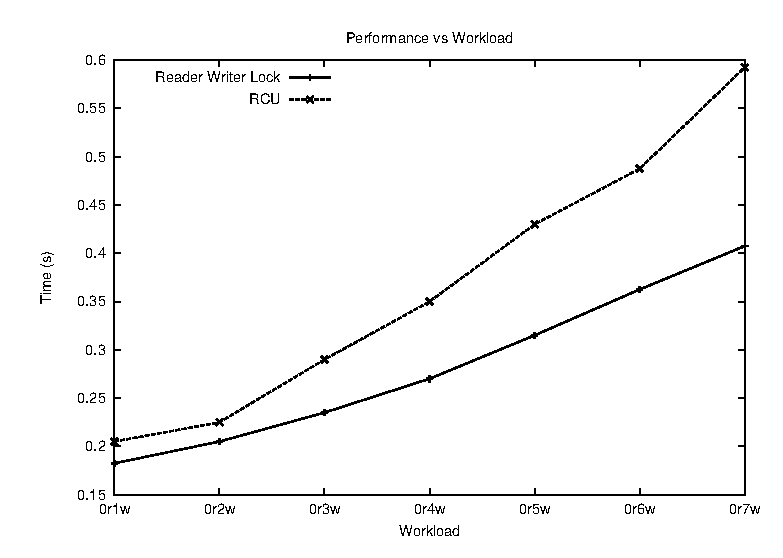
\includegraphics[scale = 0.7]{../images/graphs/macro_0r_vw}
\caption{Performance of increasing number of writers and zero readers with the 167k routing table.}
\label{img:macro_0r_vw}
\end{figure}


\begin{table}[tph]
\begin{center}
\begin{tabular}{|l|l|l|l|l|}
\hline Workload &Reader-Writer Lock (s) & RCU (s) & $\frac{\mbox{Reader-Writer Lock}}{\mbox{RCU}} $ \\
\hline 1 reader 1 writer & 2.260 & 1.540&1.468\\
\hline 1 reader 2 writers & 2.335 & 1.593&1.466\\
\hline 1 reader 3 writers & 2.397 & 1.677&1.429\\
\hline 1 reader 4 writers & 2.467 & 1.962&1.257\\
\hline 1 reader 5 writers & 2.547 & 2.078&1.226\\
\hline 1 reader 6 writers & 2.605 & 2.408&1.082\\
\hline 1 reader 7 writers & 2.663 & 2.310&1.153\\
\hline
\end{tabular}

\end{center}
\caption{Performance comparison of increasing number of writers and one reader using the 167k routing table.}
\label{tbl:macro_1r_vw}
\end{table}


\begin{figure}[tph]
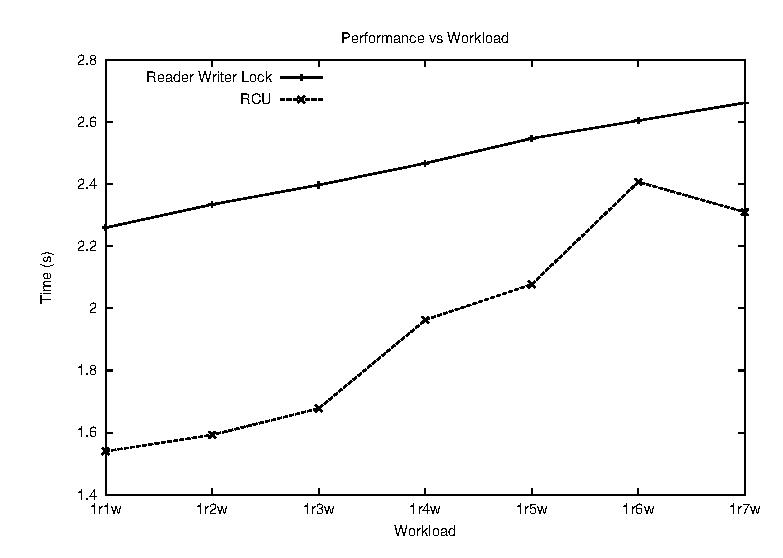
\includegraphics[scale = 0.7]{../images/graphs/macro_1r_vw}
\caption{Performance of increasing number of writers and one reader with the 167k routing table.}
\label{img:macro_1r_vw}
\end{figure}

\subsection{Micro-benchmarks}
\label{sec:microbenchmarks}
The micro-benchmarks have tests which repeatedly access a small set of addresses in a very short time span.
As with macro-benchmarks, we are interested mainly in read heavy workloads. We look at write heavy workloads for completeness.

\paragraph{Pure Reader Workload}
Here we consider a workload consisting of only readers. We look at how the reader-writer lock and RCU perform against the unmodified vanilla version.
As we can see from Table \ref{tbl:micro_vr_0w} which is represented in Figure \ref{img:micro_vr_0w}, the reader-writer lock is up to 50 times slower than a version without locks.
The reader-writer lock does not scale with an increase in the number of threads. The RCU version scales with an increase in the number of threads. The RCU version is also within 1.5 times the performance of the version without any locks.

The Reader-Writer lock spends time acquiring a lock on reads while RCU does not have any additional overhead for readers. Any additional overhead of RCU over the vanilla version is due to the overhead in checking reclaim lists and detecting quiescent states.

The Click configuration file used for this purpose is shown in Listing \ref{lst:readercomparison}.
\begin{table}
\begin{center}
\input{micro_vr_0w.tex}
\end{center}
\label{tbl:micro_vr_0w}
\caption{Performance comparison over a workload with increasing number of readers and zero writers.}
\end{table}

\begin{figure}[tph]
\fbox{
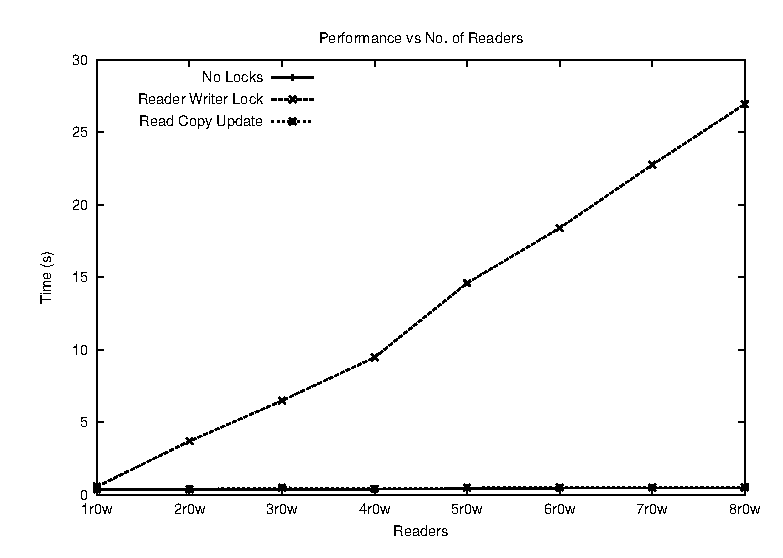
\includegraphics[scale = 0.7]{../images/graphs/micro_vr_0w}
}
\caption{Performance comparison over a workload with increasing number of readers and zero writers.}
\label{img:micro_vr_0w}
\end{figure}

\begin{lstlisting}[float=tph, caption = A Click configuration file for 4 readers, label =lst:readercomparison]
// 4 readers using the RCU (fine grained locking version)
// of RadixIPLookup.
Idle
 -> r :: RadixIPLookup106(
                1.1.1.0/32  8.1.1.1 0,
                0.0.0.0/0   8.1.1.1 0,
                ) 
 -> Idle;

reader :: ReadRadixIPLookup106(r);
reader1 :: ReadRadixIPLookup106(r);
reader2 :: ReadRadixIPLookup106(r);
reader3 :: ReadRadixIPLookup106(r);
StaticThreadSched(
        reader 0,
        reader1 1,
        reader2 2,
        reader3 3
);

DriverManager(stop);

\end{lstlisting}

\paragraph{Read Intensive workloads}
We now compare the performance of RCU over the reader-writer lock in the presence of a writer. This workload reflects typical router usage. We refer the reader to Table \ref{tbl:micro_vr_1w} and Figure \ref{img:micro_vr_1w} for the results.
RCU scales over an increase in the number of threads, however the reader-writer lock does not scale with an increase in the number of readers. This can be attributed to time spent waiting to acquire the lock before reading or writing in the Reader-Writer Lock version.

\begin{table}[tph]
\begin{center}
\input{micro_vr_1w.tex}
\end{center}
\label{tbl:micro_vr_1w}
\caption{Performance comparison of increasing number of readers with one writer.}
\end{table}

\begin{figure}[tph]
\begin{center}
\fbox{
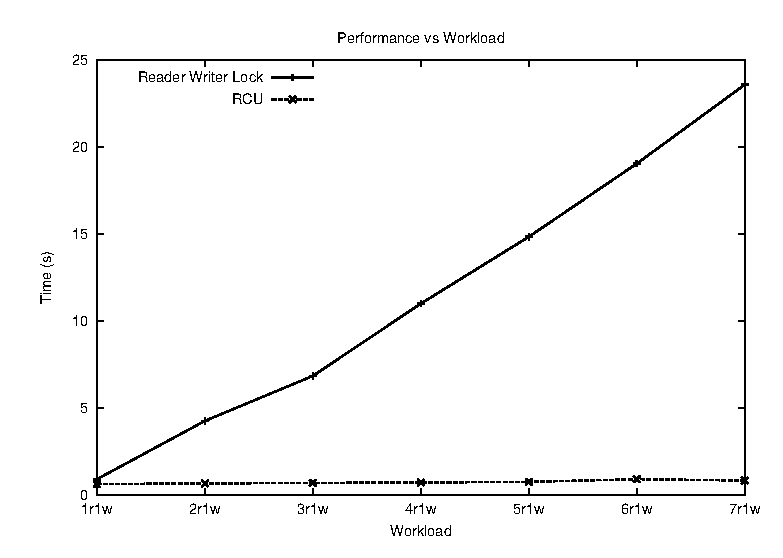
\includegraphics[scale = 0.7]{../images/graphs/micro_vr_1w}
}
\caption{Performance comparison of increasing number of readers with one writer.}
\label{img:micro_vr_1w}
\end{center}
\end{figure}

\paragraph{Write Intensive workloads}
We now compare the performance of RCU with the reader-writer lock for a write intensive workload. The performance of a workload with one reader and increasing number of writers is shown in Table \ref{tbl:micro_1r_vw} and Figure \ref{img:micro_1r_vw}. The performance of a workload with zero readers and increasing number of writers is shown in Table \ref{tbl:micro_0r_vw} and Figure \ref{img:micro_0r_vw}. In both cases, the reader-writer lock performs better than RCU. We attribute this to additional overhead caused due to lock contention to free stale data in quiescent states. When there are more writers, there is more stale data. Since these benchmarks target a very small set of routes, the reclamation also has contention for the same memory locations.

\begin{table}[tph]
\begin{center}
\input{micro_0r_vw.tex}
\end{center}
\label{tbl:micro_0r_vw}
\caption{Performance comparison of increasing number of writers with zero readers.}
\end{table}

\begin{figure}[tph]
\begin{center}
\fbox{
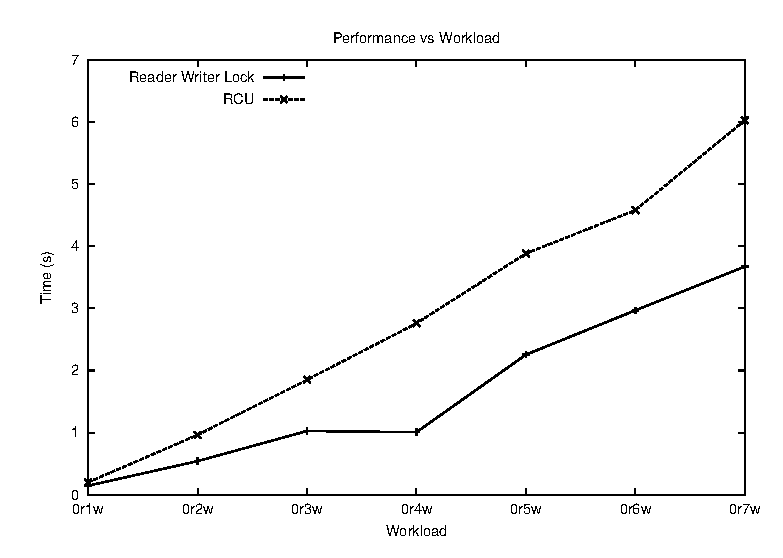
\includegraphics[scale = 0.7]{../images/graphs/micro_0r_vw}
}
\caption{Performance comparison of increasing number of writers with zero readers.}
\label{img:micro_0r_vw}
\end{center}
\end{figure}

\begin{table}[tph]
\begin{center}
\input{micro_1r_vw.tex}
\end{center}
\label{tbl:micro_1r_vw}
\caption{Performance comparison of increasing number of writers with one reader.}
\end{table}

\begin{figure}[tph]
\begin{center}
\fbox{
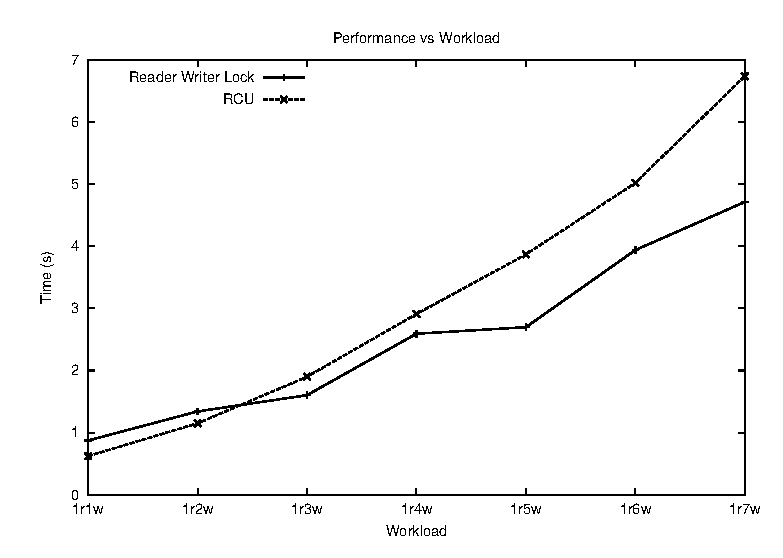
\includegraphics[scale = 0.7]{../images/graphs/micro_1r_vw}
}
\caption{Performance comparison of increasing number of writers with one reader.}
\label{img:micro_1r_vw}
\end{center}
\end{figure}


\section{Conclusion}
Lookup performance in a software router such as Click is crucially
important. Leveraging multicore processors which are available in almost all commodity hardware
today is a feasible way to improve performance. This document has outlined an efficient way to achieve a fast and safe multicore solution.


The primary challenges in implementing RCU for Click were to
identify quiescent states in a way which could be applied to all
elements. 

We have built an RCU framework for userlevel Click invlolving a
mechanism to detect quiescent states and an API which can be used by
a userlevel element in Click.

We have verified through our benchmarks that
this mechanism does indeed have a very low reader side overhead. The RCU approach is also up to 70\% better than a reader-writer lock on read intensive workloads.

\section{Future Work}

%\begin{enumerate}
%\item Implement RCU for RadixIPLookup if Radix nodes are deleted when a route is removed.
%\item Implement RCU for the Radix Tree: Currently, RCU has been only used on the vector. A coarse grained lock is acquired around updates to the Radix Tree.
%\end{enumerate}
We have experimented with the RadixIPLookup element in Click. However, it would be useful to implement a RCU based synchronization for other elements such as DirectIPLookup or RangeIPLookup.\\ 

Our approach uses RCU for the vector in RadixIPLookup, however a coarse grained lock is acquired for updates to the radix tree. The size of the radix tree depends on the size of the routing table, which is typically very large. Thus implementing RCU based synchronization for the radix tree would be very useful.
\section{Acknowledgements}
I am tremendously grateful to my advisor, Professor Eddie Kohler for his continued guidance, support and ideas.
Rohit Kumar contributed equally to this project. I am grateful to him for insightful discussions, code and comments.
\bibliography{rcu_report}
\bibliographystyle{plain}
\end{document}

